\documentclass[preprint,12pt,authoryear]{elsarticle}
\usepackage[T1]{fontenc}
\usepackage[utf8]{inputenc}
\usepackage{lmodern}
\usepackage{amsmath,amssymb}
\usepackage{graphicx}
\usepackage{booktabs,tabularx,array,adjustbox}
\usepackage[hidelinks]{hyperref}
\usepackage{xcolor}
\usepackage{float}
\usepackage{fvextra}

\DeclareUnicodeCharacter{2212}{\ensuremath{-}}
\DeclareUnicodeCharacter{2265}{\ensuremath{\geq}}
\DeclareUnicodeCharacter{2264}{\ensuremath{\leq}}
\DeclareUnicodeCharacter{00D7}{\ensuremath{\times}}
\DeclareUnicodeCharacter{2192}{\ensuremath{\rightarrow}}
\DeclareUnicodeCharacter{2190}{\ensuremath{\leftarrow}}
\DeclareUnicodeCharacter{00B1}{\ensuremath{\pm}}
\DeclareUnicodeCharacter{00B0}{\ensuremath{^\circ}}
\DeclareUnicodeCharacter{03B2}{\ensuremath{\beta}}
\DeclareUnicodeCharacter{03BB}{\ensuremath{\lambda}}
\DeclareUnicodeCharacter{2032}{\ensuremath{'}}
\providecommand{\tightlist}{\setlength{\itemsep}{0pt}\setlength{\parskip}{0pt}}
\newcommand{\pandocbounded}[1]{#1}
\setlength{\tabcolsep}{4pt}
\renewcommand{\arraystretch}{1.15}
\biboptions{sort,comma}
\journal{Computers and Electronics in Agriculture}

\usepackage{etoolbox}
\begin{document}
\begin{center}
{\Large\bfseries Supplementary Material\par}\vspace{0.6em}
{\large Certified Coverage Planning under Execution Uncertainty: Conformal Erosion with Model-Pivoted Cross-Field Calibration for Agricultural Field Operations\par}
\end{center}
\tableofcontents
\bigskip
\textbf{Names used in the manuscript and in the repository.} Experiment A1 = ``v8'' (confirmatory system comparison, fields 50--79); the exploratory comparison on fields 20--49 = ``v7''; Experiments B1--B3 = ``E-low v1--v3''; B4 = the resampling check (\texttt{docs/prereg\_validity.md}); A2, B5, C1, C2 and the cost analysis = revision experiments RV3, RV2, RV4, RV5 and RV1 (\texttt{docs/prereg\_revision.md}). Methods: XCE-T = ``CE-EVT-R'' (ratio pivot with the analytic model), XCE-MC = the same with the Monte Carlo twin; CPrP = conformal predictive programming \citep{zhao2024}; UBCP = union-bound conformal planning at pair level \citep{lindemann2023}. The extreme-value model is called ``five-layer theory'' or ``EVT'' in the repository notes. Theorem and proposition numbers in this supplement follow the manuscript.

\section*{Appendix A. Proofs and formal status of every result}
\addcontentsline{toc}{section}{Appendix A. Proofs and formal status of every result}

Items marked \emph{Remark (heuristic)} are not theorems. Results that also appear in the manuscript keep its numbers (Lemma 1, Theorem 1, Proposition 1, Theorem 2, Proposition 3, Proposition 4); results stated only here are numbered A1, A2, \ldots{} Notation follows the Nomenclature of the manuscript; in particular \(\lambda_\mathrm{ref}\) is the reference erosion, \(\nu_0,\nu_2\) are spectral moments, \(Y(x)\) is the set of executed centres at section \(x\), \(R(a)=\varphi(a)+a\Phi(a)\) is the Rice function, and \(k_\star\) is the rank of an order statistic.

\textbf{Standing assumptions.} (F1) Footprints are closed intervals of width \(w\) perpendicular to the working direction, centred on the executed position of the implement reference point; heading and hitch offsets are absorbed into that position. (F2) Misses are evaluated on the 1 m section grid; strips narrower than the grid spacing between sections are not certified. (F3) Calibration runs, deployed runs and test runs are independent given the field.

\textbf{A.1 Lemma 1 (exact covering radius).} At a section the executed footprints are the intervals \([c-w/2,c+w/2]\), \(c\in Y(x)\). The chord \([\ell,u]\) is covered iff \(\ell\) and \(u\) lie within \(w/2\) of a centre and every gap between consecutive sorted centres whose midpoint lies in the chord has half-length at most \(w/2\): the distance from a point of the chord to \(Y(x)\) is maximised at \(\ell\), at \(u\) or at an interior midpoint. Writing each term as a difference of footprint edges gives \(r^\star(x)\), and \(M=0\) iff \(\max_x r^\star(x)\le w/2\). Verified against exact interval union on the 1 m grid on every run used in this paper. \(\square\)

\textbf{A.2 Greedy planner.} The gap condition for erosion \(\lambda\) is: the extreme lateral points of the main area lie within \(w/2-\lambda\) of the outermost planned centres, and consecutive planned centres are at most \(w-2\lambda\) apart. Placing each pass as far as the gap condition allows from the previous one uses the fewest passes among placements that satisfy it (exchange argument for interval covering), and \(K(\lambda)\) is non-decreasing because the admissible spacing \(w-2\lambda\) decreases.

\textbf{A.3 Virtual erosion, Lemma A1, Theorem 1 and Corollary A1.} For a run \(e\) of the reference plan \(\pi(\lambda_\mathrm{ref})\), let \(M_\mathrm{ref}(t,e)\) be the missed area when every executed footprint has half-width \(w/2-\lambda_\mathrm{ref}+t\) (a \emph{virtual} erosion \(t\) of the executed plan; the plan is not changed). A run score \(S'\) is \textbf{valid} if \(S'(e)\le t\Rightarrow M_\mathrm{ref}(t,e)=0\) for all \(t,e\). Let \(\bar t(e)=\inf\{t:M_\mathrm{ref}(t,e)=0\}\).
\emph{Lemma A1.} If \(S'(e)<\bar t(e)\), validity at \(t=S'(e)\) gives \(M_\mathrm{ref}(t,e)=0\), so \(\bar t(e)\le t<\bar t(e)\), a contradiction; hence \(S'\ge\bar t\). \(\square\)
\emph{Theorem 1.} By Lemma 1 applied with half-width \(w/2-\lambda_\mathrm{ref}+t\), \(M_\mathrm{ref}(t,e)=0\) iff \(\max_xr^\star(x)\le w/2-\lambda_\mathrm{ref}+t\), i.e.~iff \(S^\star(e)\le t\). Hence \(S^\star=\bar t\) exactly, with no assumption, and \(S^\star\le S'\) for every valid \(S'\). \(\square\)
\emph{Corollary A1.} Order statistics are monotone under pointwise order, so \(S^\star_{(k_\star)}\le S'_{(k_\star)}\) for every calibration sample and every rank \(k_\star\); because \(K(\lambda)\) is non-decreasing, a rule that deploys \(\pi(S^\star_{(k_\star)})\) deploys no more passes than the same rule applied to \(S'\). Reading the virtual erosion of the reference plan as the needed erosion of \emph{another} plan is the transfer step of A.7 and A.15; Theorem 1 and Corollary A1 do not depend on it. For CE+ with a non-constant normaliser the pointwise dominance holds for \(S/\sigma(z)\) only when \(\sigma\) is constant. \(\square\)
\emph{Numerical check.} On 6 fields × 200 runs in three regimes: \(\{M>0\}=\{S^\star>\lambda_\mathrm{ref}\}\) on 100\% of runs and \(S^\star\le S_\mathrm{pair}\) on 100\% of runs; the gap between the two at the 0.9 quantile was 0.4--1.3 cm under RTK and 5.5--9.2 cm under DGPS.

\textbf{A.4 What CE guarantees.} CE deploys \(\pi(\lambda_\mathrm{ref})\) only if the fresh certificate quantile satisfies \(q^\star\le\lambda_\mathrm{ref}\), and refuses otherwise. By Lemma 1 the deployed plan is miss-free iff its run score is at most \(\lambda_\mathrm{ref}\). Under exchangeability of the certificate batch and the test run, the marginal rule gives \(P(\text{deploy and miss})\le P(S_\mathrm{new}>q^\star)\le\varepsilon\); a statement conditional on deployment needs the PAC rule, which gives \(P(S_\mathrm{new}>\lambda_\mathrm{ref}\mid\text{calibration})\le\varepsilon\) on an event of probability at least \(1-\delta\), and deployment is a function of calibration. The pilot batches that choose \(\lambda_\mathrm{ref}\) are discarded, so the certificate batch is not selected. \(\square\)

\textbf{A.5 Lemma A3 (union bounds are looser).} If run \(i\) has \(\max_jS'_{ij}>\max_jq_j\), some \(j\) has \(S'_{ij}>q_j\). Each \(q_j\) at level \(\varepsilon/J\) admits at most \(n\varepsilon/J\) exceedances, so at most \(n\varepsilon\) runs exceed \(\max_jq_j\): \(\max_jq_j\) is at least the joint empirical \((1-\varepsilon)\) quantile. The conformal version with \(k_j=\lceil(n+1)(1-\varepsilon/J)\rceil\) satisfies the same inequality. \(\square\)

\textbf{A.6 Proposition 1 (nominal-plan calibration does not transfer).} Counterexample: let the pair scores of every plan be i.i.d. with continuous distribution \(G\), and let \(\pi(0)\) have \(K_0\) pairs and \(\pi(\hat\lambda)\) have \(K_1>K_0\). Calibrating the maximum of \(K_0\) scores at level \(1-\varepsilon\) gives a threshold \(t\) with \(G(t)^{K_0}\approx1-\varepsilon\), at which the deployed plan has coverage \(G(t)^{K_1}\approx(1-\varepsilon)^{K_1/K_0}<1-\varepsilon\). No distribution-free statement can hold for every \(G\). \(\square\)

\textbf{A.7 Theorem A1 (multiplicative transfer).} \emph{Coupling lemma.} If \(J(\pi_1)\subseteq J(\pi_0)\) under a pairing map of (pair, section) index sets, then \(\{U_{\pi_1}>t\}\subseteq\{U_{\pi_0}>t\}\cup\bigcup_{j\in J(\pi_1)}\{t-h_j<T_j^{(0)}\le t\}\): if \(T_j^{(1)}>t\) then either \(T_j^{(0)}>t\) or \(t\ge T_j^{(0)}\ge T_j^{(1)}-h_j>t-h_j\). \emph{Hazard lemma.} \(P(t-h<T\le t)=\bar F(t-h)-\bar F(t)\le(e^{hH}-1)\bar F(t)\). \emph{Extremal-index identity.} \(\sum_jP(T_j^{(0)}>t)=\mathbb EN_t=(1-F_{\pi_0}(t))/\theta_t\). Combining the three gives \(1-F_{\pi_1}(t)\le c(t)(1-F_{\pi_0}(t))\) with \(c(t)=1+(e^{hH}-1)/\theta_t\). \emph{Deployment.} \(\hat\lambda\) is random and \(c\) depends on it, so the marginal rule gives \(P(\text{miss})=\mathbb E[1-F_{\pi_1}(\hat\lambda)]\le\sup_{t\le\lambda_\mathrm{ref}}c(t)\,\varepsilon\) on the event \(\hat\lambda\le\lambda_\mathrm{ref}\); the PAC rule gives the conditional bound \(c(\hat\lambda)\varepsilon\) with probability at least \(1-\delta\). \(\square\)

\textbf{A.8 Proposition A1 (price of an inflated reference plan).} \(\{U_{\pi_1}\le t<U_{\pi_0}\}\) implies that one of the \(a=|J(\pi_0)\setminus J(\pi_1)|\) extra reference pairs exceeds \(t\). With identically distributed pairs and \(h=0\), a union bound and the extremal-index identity give \(F_{\pi_1}(t)-F_{\pi_0}(t)\le\frac{a}{|J(\pi_0)|}\cdot\frac{1-F_{\pi_0}(t)}{\theta_t}\). With \(K(\lambda)\propto1/(w-2\lambda)\), \(a\approx K(\hat\lambda)\cdot2(\lambda_\mathrm{ref}-\hat\lambda)/(w-2\lambda_\mathrm{ref})\). For R1 (\(\varepsilon=0.1\), \(\lambda_\mathrm{ref}-\hat\lambda\approx5\) cm, \(w=3\) m) and the measured range \(\theta_t\in[0.30,0.66]\) this is about 0.5--1.2 percentage points of over-coverage. \(\square\)

\textbf{A.9 Proposition A2 (training-only gating).} The selected normalisation is a function of training fields only, hence independent of calibration and test runs; conditionally on it, \((S_i,z_i)\) of calibration and test runs are exchangeable, so \(S_i/\sigma(z_i)\) are exchangeable and the split-conformal lemma applies to the score on the reference plan. The deployed plan \(\pi(t\,\sigma(z_\mathrm{new}))\) is random through \(z_\mathrm{new}\), which is correlated with the test run's condition; the pathwise transfer of A.15 still applies, and the bound becomes \(P\big(S_\mathrm{new}>t\,\sigma(z_\mathrm{new})-\bar\Delta\big)\) rather than \(\kappa\varepsilon\). \(\square\)

\textbf{A.10 Proposition A3 (conditional Gaussianity).} \emph{Additional assumption (A3):} the closed-loop state at the start of each pass is either reset or part of \(C\); equivalently, state carried through a headland turn (integrator, slip, heading, steering) is treated as a known initial condition. Under the time-invariant linear model L1 with Gaussian innovations independent across passes, a linear system with Gaussian input has a Gaussian state; \(\rho(A)<1\) gives a unique positive semidefinite Lyapunov solution; \(de/dx=\psi+\beta\) gives \(\nu_2=P_{\psi\psi}+2P_{\psi\beta}+P_{\beta\beta}\). A pair gap \((e_{k+1}-e_k)/2\) has variance \(\nu_0/2\); a single-pass edge process has variance \(\nu_0\). The plan enters only through the mean \textbf{for the time-invariant L1}; the refinements of Appendix B.1 (pass-specific observation weights, linearisation along a plan-dependent trajectory, describing functions that depend on the mean) make the covariance plan-dependent, so in the model actually used Proposition A3 holds only approximately. \(\square\)

\textbf{A.11 Theorem A2(a) (Kac--Rice).} \(\{\sup Z>t\}\subseteq\{Z(0)>t\}\cup\{N_t^+\ge1\}\), so \(\mu_j\le P(Z(0)>t)+\mathbb EN_t^+\). For a Gaussian process with \(C^1\) paths satisfying the Kac--Rice regularity conditions (Azaïs and Wschebor, 2009, Thm 3.4), \(\mathbb EN_t^+=\int\mathbb E[(Z')^+\mid Z=t]\,p_{Z(x)}(t)\,dx\); conditionally on \(Z(x)=t\), \(Z'(x)\) is Gaussian with mean \(\tilde m'(x;t)=m_j'(x)+r(x)(t-m_j(x))/s(x)^2\) and standard deviation \(\tilde s'(x)=\sqrt{s'(x)^2-r(x)^2/s(x)^2}\), so \(\mathbb E[(Z')^+\mid Z=t]=\tilde s'R(\tilde m'/\tilde s')\). The discrete version follows from \(\{\max_iZ_i>t\}\subseteq\{Z_0>t\}\cup\bigcup_i\{Z_i\le t<Z_{i+1}\}\). Tail exactness (ratio → 1 as \(t\to\infty\)) needs a finite second factorial moment of the number of upcrossings; the slip component is an Ornstein--Uhlenbeck process, so \(Z\) is \(C^1\) but not \(C^2\), and only the discrete version is used numerically. In the development checks the continuous version was about 29\% loose at the 0.9 quantile and the discrete version 0--17\%. \(\square\)

\textbf{A.12 Theorem A2(b) (field-edge terms).} Fix \(C\) and a section with chord end \(b\). Let \(\mathcal K_b\) be the passes whose planned footprint covers \(b\). If \(b\) is missed, every pass in \(\mathcal K_b\) has receded from \(b\), i.e.~\(E_k>t\) for all \(k\in\mathcal K_b\) with \(E_k\) the single-pass edge process; hence \(\{b\text{ missed at }t\}\subseteq\bigcap_{k\in\mathcal K_b}\{E_k>t\}\) (passes outside \(\mathcal K_b\) can only rescue the edge, so this is an inclusion, not an identity). Given \(C\) and under A3, the random parts of different passes are independent, so \(P(\cdot\mid C)\le\prod_{k\in\mathcal K_b}P(E_k>t\mid C)\). Sections covered by one pass use the discrete bound of (a) or Gaussian Monte Carlo; sections covered by two passes are combined across \(x\) by a union bound, which is valid but can be loose. The result is an upper bound on the edge exceedance and enters L3 as a boundary pseudo-pair. \(\square\)

\textbf{A.13 Theorem A3 (Bonferroni sandwich).} First- and second-order Bonferroni inequalities give \(1-\Lambda\le P(\cap_jA_j^c\mid C)\le1-\Lambda+\sum_{i<j}P(A_i\cap A_j\mid C)\) with \(\Lambda=\sum_j\mu_j\). Non-adjacent pairs are independent given \(C\) (A3), so \(P(A_i\cap A_j\mid C)=\mu_i\mu_j\) for \(|i-j|\ge2\), and \(p_j\le\min(\mu_j,\mu_{j+1})\). The alternating expansion of \(\prod_j(1-\mu_j)\) gives \(1-\Lambda\le\prod_j(1-\mu_j)\le1-\Lambda+\sum_{i<j}\mu_i\mu_j\). Both quantities lie in an interval of length at most \(\eta=\Lambda^2/2+\sum_j\min(\mu_j,\mu_{j+1})\). \textbf{Status.} The second term of \(\eta\) is first order in \(\Lambda\): for \(J\) homogeneous pairs it equals \(\Lambda(J-1)/J\), i.e.~about 0.10--0.11 at the certified level (\(\Lambda\approx0.105\), \(J=10\)--\(50\)). The bound is therefore not informative at \(1-\varepsilon=0.9\); the accuracy of the product form is established empirically (Table S5: 0.888, 0.882 and 0.900 against a true 0.900), not by Theorem A3. A sharper bound would bound \(p_j\) as a bivariate Gaussian exceedance with same-section correlation \(-\tfrac12\). \(\square\)
\emph{Correlation of adjacent pairs.} With equal single-pass variances \(\sigma^2\) and autocorrelation \(r(x,x')\), \(\mathrm{Cov}(Z_j(x),Z_{j+1}(x'))=-\tfrac14\sigma^2r(x,x')\) and \(\mathrm{Var}\,Z_j=\tfrac12\sigma^2\), so \(\rho_{xx'}=-\tfrac12r(x,x')\); the single-pass autocorrelation is about \(-0.24\) at 10 m because of the integral action (the loop is not under-damped; \(\zeta\approx0.70\)), so the correlation changes sign with lag and neither Slepian's inequality nor a small-correlation comparison applies. With pass-specific variances (B.1(a)) these values hold approximately.

\textbf{A.14 Lemma A2 (mixed representation) and the extremal index.} Integrate Theorem A3 over \(C\): \(F_\pi(t)=\mathbb E_C[\prod_j(1-\mu_j)]+\rho_\pi(t)\) with \(|\rho_\pi|\le\mathbb E_C[\eta]\). For the extremal index, with \(1-F_\pi\approx\mathbb E_C[1-e^{-\Lambda}]\) and \(\mathbb EN_t=\mathbb E_C[\Lambda]\), \(\theta_t\approx\mathbb E_C[1-e^{-\Lambda}]/\mathbb E_C[\Lambda]\). Since \(1-e^{-x}<x\), \(\theta_t<1\) even for a constant \(\Lambda\) (0.949 at \(\Lambda=0.105\)); by Jensen, \(\theta_t\le(1-e^{-\mathbb E\Lambda})/\mathbb E\Lambda\), and variation of \(\Lambda\) between operating conditions lowers \(\theta_t\) further. The measured values (0.30--0.66) are far below the homogeneous value, which points to heterogeneity across conditions; the Poisson approximation given \(C\) ignores adjacent-pair dependence, so this attribution is indicative, not proven. \(\square\)

\textbf{A.15 Theorem 2 (transfer under superposition).} \emph{Hypothesis (S).} Couple the reference plan \(\pi_0\) and the deployed plan \(\pi_1\) by sharing the operating condition \(C\) and the per-pass noise \(\xi_k\), and pair their (pass pair, section) index sets by a map under which \(J(\pi_1)\subseteq J(\pi_0)\). Assume that for coupled realisations the matched gap and edge processes differ by a term that does not depend on the noise: \(Z^{(1)}_j(x)-Z^{(0)}_j(x)=d_j(x;C)\le\Delta(C)\le\bar\Delta\), where \(d_j\) includes the geometric difference of the edge terms. (S) holds exactly for a linear closed loop (superposition of the response to the deterministic input and to the noise) and approximately for the simulator. \emph{Proof.} Under (S), \(\{T^{(1)}_j>t\}\subseteq\{T^{(0)}_j>t-\Delta(C)\}\) for every \(j\in J(\pi_1)\), so \(\{U_{\pi_1}>t\}\subseteq\{U_{\pi_0}>t-\Delta(C)\}\subseteq\{U_{\pi_0}>t-\bar\Delta\}\) pathwise. Taking probabilities, \(1-F_{\pi_1}(t)\le1-F_{\pi_0}(t-\bar\Delta)=\kappa(t)(1-F_{\pi_0}(t))\). Gaussianity is not needed. \emph{Deployment.} The marginal rule gives \(P(\text{miss})\le\sup_{t\le\lambda_\mathrm{ref}}\kappa(t)\,\varepsilon\) on \(\{\hat\lambda\le\lambda_\mathrm{ref}\}\); if \(1-F_{\pi_0}\) is log-concave on the relevant range, \(\kappa\) is non-decreasing and the supremum is \(\kappa(\lambda_\mathrm{ref})\). The PAC rule gives \(\kappa(\hat\lambda)\varepsilon\) conditionally, with probability at least \(1-\delta\). \emph{Closed form.} If \(1-F\propto Q(u)\) near the threshold with standard deviation \(s\), \(\log Q(u-d)-\log Q(u)\le d\,\vartheta(u)\le d(u+1/u)\) for \(u\ge1\), because the Gaussian hazard \(\vartheta=\varphi/Q\) is increasing and \(\vartheta(u)\le u+1/u\); under a mixture over \(C\) take the supremum over \(C\) of the per-condition bound. \emph{Mean shift.} With integral action, after the transient that follows each headland turn, \(\Delta_j\le\tfrac12h_a(1-c_{\min})\sup_x|\Delta g^{(1)}_j(x)-\Delta g^{(0)}_j(x)|\) plus a GNSS timing term bounded by the modulus of continuity of the error series. \(\square\)

\textbf{A.16 Remark (Gumbel scale law; heuristic).} For one stationary Gaussian process with constant mean \(m\), standard deviation \(s\) and effective length \(L\), the Cramér--Leadbetter theorem (Leadbetter et al., 1983, Thm 8.2.7) gives a Gumbel limit and, inverting at \(1-\varepsilon\), \(t_\varepsilon\approx m+s[a_L-\log(-\log(1-\varepsilon))/a_L]\) with \(a_L=\sqrt{2\log L}\). Applying it to the maximum over \(K\) dependent pair processes and edge processes (variance \(\nu_0\) instead of \(\nu_0/2\)) is not proven, and edge processes can dominate as \(L\to\infty\). A tenfold larger field raises \(a_L\) by about 15.5\% and \(t_\varepsilon/s\) (at \(m=0\)) by about 11\% for \(L\sim10^3\). Normal extremes converge at rate \(O(1/\log L)\) \citep{hall1979}. The law is used only to motivate the scale-law comparator pivot.

\textbf{A.17 Proposition 3 (cross-field validity).} Assume fields \(f_1,\dots,f_n,g\) are exchangeable (i.i.d. for the PAC statement), each calibration field contributes one run at its reference plan, and \(\hat q_f\in(0,\infty]\) is a measurable function of field \(f\) only. Then \(V_i=S_i/\hat q_{f_i}\) and \(V_\mathrm{new}\) are exchangeable (ties at \(+\infty\) allowed), \(S_\mathrm{new}\le\hat q_gv^\star\iff V_\mathrm{new}\le v^\star\), and the split-conformal lemma gives \(P(S_\mathrm{new}\le\hat q_gv^\star)\ge k_\star/(n+1)\ge1-\varepsilon\) (marginal), or the PAC statement. This is a guarantee on the \textbf{score at the reference plan}; for the deployed plan \(\pi_g(\hat q_gv^\star)\) it becomes \(\sup\kappa\cdot\varepsilon\) by A.15 when \(\hat q_gv^\star\le\lambda_\mathrm{ref}\). A deployment capped below the conformal threshold (as in the resampling checks, where an infinite threshold was replaced by the planner cap) is not covered and is reported separately. The coverage given the calibration set is \(H(v^\star)\), a population average over target fields, which is \(\mathrm{Beta}(k_\star,n+1-k_\star)\) under exchangeability; a single field's coverage is not. \(\square\)

\textbf{A.18 Remark (ratio versus PIT pivot; heuristic).} See Appendix B.4.

\textbf{A.19 Proposition A4 (per-field validity criteria).} For 200 test runs, a field fails the one-sided binomial test at 0.05 iff at most 172 runs are miss-free; with true coverage exactly 0.9 this has probability 0.043. Given \(n=100\) calibration runs, the coverage of the marginal rule (\(k_\star=91\)) is Beta(91, 10), and of the PAC rule (\(k_\star=95\)) Beta(95, 6); integrating the binomial failure probability gives 14.5\% and 1.2\%. A PAC method is declared invalid if 9 or more of 30 fields fail (\(P(\mathrm{Bin}(30,0.143)\ge9)=0.021\) under the general upper bound \(\delta+\alpha=14.3\%\)). \(\square\)

\textbf{A.20 Proposition 4 (margin inflation under the ideal scale).} Under the ideal pivot \(q_f=\lambda^\star_f\) the \(V_i\) are i.i.d. with distribution \(H\), and \(H(V_{(k_\star)})\sim\mathrm{Beta}(k_\star,n+1-k_\star)\); \(\lambda_g/\lambda^\star_g=V_{(k_\star)}\) does not depend on \(g\). If normalised shapes coincide, \(V_{(k_\star)}=\Gamma^{-1}(B)\). \textbf{This is an identity for the ideal pivot, not a lower bound over all pivots:} another pivot changes both the between-field spread and \(H\), and in the R3 PAC cell raw pooling was cheaper than the ideal pivot (+10.36 vs +12.86 pp). \emph{Prediction.} Replacing \(G_f\) by the theory CDFs, drawing one run per field, normalising and taking the PAC order statistic 2000 times gives the predicted inflations of Fig. 7. \(\square\)

\section*{Appendix B. Theory details}
\addcontentsline{toc}{section}{Appendix B. Theory details}

\subsection*{B.1 Refinements of L1 forced by failed validation checks}
\addcontentsline{toc}{subsection}{B.1 Refinements of L1 forced by failed validation checks}

\begin{enumerate}
\def\labelenumi{(\alph{enumi})}
\item
  \emph{Observation operator.} Misses are evaluated on offsets linearly interpolated to a 1 m grid with a pass-constant weight \(f_k\), so \(\mathrm{Var}\,\tilde e_k=(1-f)^2v_s+f^2v_{s+1}+2f(1-f)c_s\) (exact form). An earlier stationary approximation produced a negative variance on one R3 field, which caused the E-low v1 failure in R3. Ignoring the operator overestimates variance by 2--3\% and tail probability by 15--30\%.
\item
  \emph{Time-varying quasi-linearisation} along the noise-free closed-loop trajectory, with Jacobians of the kinematics and terrain feedback and random-input describing functions for steering saturation and rate limits \citep{booton1954,kazakov1956}; covariance propagates by \(P_{t+1}=A_tP_tA_t^\top+B_tB_t^\top\).
\item
  \emph{Integrator clamp.} The anti-windup clamp \(|I|\le0.3\) sits about 1.6 standard deviations from zero; it is replaced by a leaky integrator whose leak rate matches the stationary variance of the truncated Gaussian (Kazakov-type energy criterion). This is a best estimate; the unclamped linear model is a safe upper bound because clamping only reduces variance. In the three test conditions of the integrator model, the true variance lay between the best estimate and the safe upper bound.
\end{enumerate}

\emph{Assumption on terrain.} The simulator samples slope by nearest neighbour on a 1 m grid; at high slip, crossing a grid boundary makes slip jump, and the conditional distribution is no longer Gaussian. The theory therefore assumes a terrain gradient that is smooth on the operating scale (A1′); changing the simulator would break comparability with existing experiments and is left to a separate validation.

\subsection*{B.2 Layer-by-layer validation (developmental)}
\addcontentsline{toc}{subsection}{B.2 Layer-by-layer validation (developmental)}

Development fields: R1 wheat 440, R2 paddy 36 (144 passes), R3 paddy 40; L5 on 8 R1 fields.

\begin{table}[!htbp]
\centering
\footnotesize
\renewcommand{\thetable}{S5}\caption{Layer-by-layer validation after the first round of corrections (developmental).}
\begin{adjustbox}{max width=\textwidth}
\begin{tabular}{@{}l>{\raggedright\arraybackslash}p{20.8em}>{\raggedright\arraybackslash}p{20.8em}>{\raggedright\arraybackslash}p{13.5em}l@{}}
\toprule
\textbf{Layer} & \textbf{Quantity} & \textbf{R1 flat RTK} & \textbf{R2 hilly-wet RTK} & \textbf{R3 DGPS} \\
\midrule
1 & RMS difference, noise-free closed-loop mean vs conditional sample mean & 0.07 cm & 0.20 cm & 0.09 cm \\
1 & Pair standard deviation, sample / predicted & 1.00 & 0.999 (5--95\%: 0.989--1.015) & agrees \\
1 & Adjacent-section covariance, sample / predicted & --- & 0.993 & --- \\
3 & Product form for \(P(U\le t\mid C)\) at the 0.9 quantile (predicted / true) & 0.888 / 0.900 & 0.882 / 0.900 & 0.900 / 0.900 \\
4 & Coverage after a plan change, predicted / simulated & 0.901 / 0.899 & 0.890 / 0.885 & 0.920 / 0.922 \\
5 & Linearity of \(q_{0.9}\) in \(\sqrt{2\log N}\) over 8 fields & simulated \(R^2=0.989\), predicted \(R^2=0.964\); per-field error 0.1--0.7 cm & --- & --- \\
\bottomrule
\end{tabular}
\end{adjustbox}
\end{table}

\begin{table}[!htbp]
\centering
\footnotesize
\renewcommand{\thetable}{S5a}\caption{Required margin \(q_{0.9}\) (cm), predicted / simulated, all development versions (the first manuscript version showed the first and final versions).}
\begin{adjustbox}{max width=\textwidth}
\begin{tabular}{@{}ll>{\raggedright\arraybackslash}p{7.3em}>{\raggedright\arraybackslash}p{10.9em}>{\raggedright\arraybackslash}p{7.3em}@{}}
\toprule
\textbf{Regime} & \textbf{First version} & \textbf{Fix 1 (product form, time-varying L1)} & \textbf{Fix 2 (integrator, hybrid exact L2)} & \textbf{Safe upper bound} \\
\midrule
R1 flat RTK & 11.03 / 11.01 & 11.02 / 11.01 & 10.94 / 11.01 (−0.6\%) & 11.02 \\
R2 hilly-wet RTK & 15.75 / 15.26 & 15.76 / 15.26 & 15.39 / 15.26 (+0.9\%) & 15.76 \\
R3 DGPS & 36.0 / 37.09 (−2.9\%) & 37.97 / 37.09 & 37.61 / 37.09 (+1.4\%) & 37.97 \\
\bottomrule
\end{tabular}
\end{adjustbox}
\end{table}

After fix 2, coverage after a plan change is predicted to within 0.007 (R3: 0.9220 vs 0.9220). The extremal index agrees in R2 (0.30 vs 0.31) but is underpredicted in R3 (0.54 vs 0.66), which does not affect \(F_\pi\) (A.14). A diagnostic in the hardest condition (R2, slip gain 1.23) showed conditional marginals that are Gaussian (skewness −0.002, excess kurtosis −0.012), and a Gaussian model with \emph{sample} moments reproduced the simulated exceedance (0.1105 vs 0.1033), while L1's moments before the integrator fix overstated it by 25\%; the residual bias was in L1's moments, which the integrator model removed.

\emph{Product form versus \(e^{-M}\)} at a fixed DGPS condition (true no-miss probability / \(e^{-M}\) / product): 0.3000 / 0.4851 / 0.2988 at the 0.3 quantile; 0.5000 / 0.6033 / 0.4999 at 0.5; 0.9000 / 0.9048 / 0.9000 at 0.9 (source: docs/theory\_evt.md §3). Per-condition diagnostic in R3 (400 conditions × 4 runs): for the conditions that miss, predicted no-miss 0.220 before and 0.028 after the correction against 0.045 observed; overall 0.919 before, 0.900 after, 0.900 observed.

\subsection*{B.3 Development of the field-edge terms (post hoc)}
\addcontentsline{toc}{subsection}{B.3 Development of the field-edge terms (post hoc)}

The edge terms of Theorem A2(b) went through three versions, each checked against the empirical 0.9 quantile of 200 independent runs on the reference plan (\texttt{scripts/check\_boundary.py}):

\begin{enumerate}
\def\labelenumi{\arabic{enumi}.}
\tightlist
\item
  Taking the \emph{lowest} covering pass as the binding one overestimated the edge contribution about twofold: when the edge lies in the overlap band of two passes, the selected pass is about to lose coverage while its neighbour still covers the edge.
\item
  Taking the single covering pass with the centre \emph{nearest} to the edge still overestimated by about 14\%: inside an overlap band both passes must move apart for a miss, which common-mode error rarely produces.
\item
  The reported version takes the product of the two single-pass probabilities in overlap bands.
\end{enumerate}

Per-field results of the final version (theory without edges \(q_\mathrm{old}\), with edges \(q_\mathrm{new}\), simulated 0.9 quantile, all in m):

\begin{table}[!htbp]
\centering
\footnotesize
\renewcommand{\thetable}{S5b}\caption{Field-edge terms on the 15 E-low v3 R3 test fields. log(\(q\)/sim): without edges mean −0.040, sd 0.108; with edges mean +0.008, sd 0.106. On 4 R1 fields: +0.003 / 0.048 → +0.004 / 0.048; on 4 R2 fields: +0.009 / 0.046 → +0.018 / 0.047 (results/lowdata\_v3/check\_boundary\_R1\_R2.txt). The edge terms raise the prediction most on fields with few passes (e.g.~7--13 passes), where the boundary is a larger share of the field.}
\begin{adjustbox}{max width=\textwidth}
\begin{tabular}{@{}lllll@{}}
\toprule
\textbf{R3 field} & \textbf{Passes} & \textbf{\(q_\mathrm{old}\)} & \textbf{\(q_\mathrm{new}\)} & \textbf{Simulated} \\
\midrule
119 & 18 & 0.322 & 0.322 & 0.298 \\
54 & 20 & 0.485 & 0.499 & 0.387 \\
32 & 15 & 0.346 & 0.346 & 0.400 \\
44 & 24 & 0.334 & 0.340 & 0.338 \\
212 & 11 & 0.368 & 0.391 & 0.395 \\
74 & 23 & 0.382 & 0.390 & 0.398 \\
211 & 21 & 0.321 & 0.329 & 0.327 \\
181 & 14 & 0.304 & 0.323 & 0.372 \\
24 & 10 & 0.335 & 0.357 & 0.397 \\
182 & 20 & 0.378 & 0.381 & 0.372 \\
215 & 7 & 0.288 & 0.300 & 0.319 \\
225 & 12 & 0.352 & 0.407 & 0.333 \\
28 & 13 & 0.403 & 0.424 & 0.430 \\
48 & 8 & 0.299 & 0.363 & 0.349 \\
21 & 15 & 0.386 & 0.388 & 0.381 \\
\bottomrule
\end{tabular}
\end{adjustbox}
\end{table}

\textbf{Scope.} E-low v1--v3 and v8 pre-registered results used the theory without edge terms. Validity is unaffected, because the guarantee comes from exchangeability, not from theory accuracy; only R3 efficiency comparisons could change.

\subsection*{B.4 Ratio versus probability-integral-transform pivot (Remark; heuristic, motivated post hoc)}
\addcontentsline{toc}{subsection}{B.4 Ratio versus probability-integral-transform pivot (Remark; heuristic, motivated post hoc)}

Let the theory be exact up to a scale error, \(\hat F_f(t)=F_f(t/(1+\delta_f))\).

\begin{itemize}
\tightlist
\item
  \emph{Ratio pivot:} \(\hat q_f=(1+\delta_f)q_f\), so \(V_f=S_f/((1+\delta_f)q_f)\) and \(\lambda_g=(1+\delta_g)q_gv^\star\). The deployed margin is affected linearly, \(\partial\lambda_g/\partial\delta_g=q_gv^\star\), and the theory is evaluated only at the \((1-\varepsilon)\) quantile, which L1--L4 predict most accurately.
\item
  \emph{PIT pivot:} \(\lambda_g=\hat F_g^{-1}(v^\star)\) with \(v^\star\) close to 1, and \(\partial\lambda_g/\partial v^\star=1/\hat f_g(\lambda_g)\). In the tail \(\hat f_g\to0\), so small errors in \(v^\star\) (from tail errors of \(\hat F_{f_i}\) on calibration fields) become large errors in \(\lambda_g\). With the PAC rule at \(n\approx30\), \(v^\star\) is near the largest PIT value, where this amplification is strongest. A non-finite \(\hat F\) is additionally sorted to the top and drives \(v^\star\) to the extreme tail (observed in E-low v1, R3).
\end{itemize}

Under the corrected theory in E-low v2, R3 PAC: the PIT pivot's excess overlap was +28.38 pp against +15.25 pp for the ratio pivot (Table S8).

\section*{Appendix C. Experimental details}
\addcontentsline{toc}{section}{Appendix C. Experimental details}

\subsection*{C.1 Simulator}
\addcontentsline{toc}{subsection}{C.1 Simulator}

Vectorised over runs, \(\Delta t=0.05\) s, speed 2 m/s. Kinematics \(\dot d=v\sin(\psi+\beta)\), \(\dot\psi=v\tan\delta/l\); first-order steering lag \(\tau=0.25\) s with 35° saturation and 30°/s rate limit; terrain slip \(\beta=-0.35\,k_s\,g_\mathrm{lat}\) plus Ornstein--Uhlenbeck roughness, with \(k_s\) and roughness set by per-run soil moisture; antenna height 2.6 m with roll-compensation factor \(c=0.85\pm0.05\); per-run mounting bias with \(\sigma=1.5\) cm; GNSS error projected on the lateral axis, with passes executed in real time order including headland turns. Controllers: pure pursuit, Stanley, LQR and LQR with integral action (LQR-I, default, designed on the delay-augmented model, with conditional-integration anti-windup); external controllers plug into the same interface.

GNSS processing: the first 30 min of each day is removed; truth is IGS20/ITRF2020 coordinates propagated to the epoch; 30 s epochs are interpolated to 1 Hz and high-frequency residuals from the i2Nav vehicle dataset \citep{tang2022} are added. CitrusFarm RTK robot logs \citep{teng2023}, 123 rows, are available for offline replay (\texttt{results/real.csv}, \texttt{results/real\_aci.csv}; not summarised).

\subsection*{C.2 Field splits}
\addcontentsline{toc}{subsection}{C.2 Field splits}

Fields are ordered by \texttt{core.load\_fields(seed=0)}. Indices 0--4: training fields (CE+ fitting, farmer tuning, reference erosion). 5--19: earlier system experiments v3--v6 (which answer a different question with target-field data) and the E-low v3 test fields; no E-low design or analysis used them before E-low v3. 20--49: v7 system comparison. 50--79: v8 confirmatory system comparison, E-low v2 test fields and the E-low v3 calibration pool (the v8 method choice was fixed before E-low v2). 80 onward: E-low v1, all exploratory analyses that led to E-low v2, and the E-low v3 training pool (gate and CQR fitting only). The resampling check (manuscript Section 6.4, Experiment B4) reuses the v2 and v3 fields with new historical-run banks.

\subsection*{C.3 Baselines}
\addcontentsline{toc}{subsection}{C.3 Baselines}

About 25 published or industry systems, each implemented as a plug-in module. Where the publisher full text was not accessible, the implementation follows the abstract and secondary descriptions, and the module says so: Hameed 3D terrain spacing, the Lenain slip-observer controller, the Gaussian-belief models and the ISO pass-to-pass definition behind the vendor rule. The conformal planners are our adaptations to the coverage problem: CPrP and UBCP calibrate their own scores (pair score; per-pair quantiles with a union bound) on the nominal plan, as their original formulations do; UBCP pools scores across pairs by default, which loses its finite-sample guarantee (stated in the code); and the PAC version of UBCP, which also splits \(\delta\) over constraints, is our construction. The scenario approach and Wasserstein DRO run at confidence \(\beta=0.01\), not \(\delta=0.1\), and the DRO radius is a heuristic, untuned choice, so these two are not compared within a guarantee class. Systems: vendor-specification overlap (twice the nominal pass-to-pass accuracy) and farmer-tuned global overlap (tuned once on the training fields to P(no miss) ≥ 0.9), with and without vendor terrain compensation; Fields2Cover \citep{mier2023}, Hameed 3D terrain spacing \citep{hameed2016} and follow-previous-pass guidance as planners; Lenain-type slip-observer control \citep{lenain2006}, ESO sliding-mode control and offset-free MPC \citep{pannocchia2003} as controllers; tube-MPC radius margin \citep{mayne2005}; Gaussian chance constraints (pointwise, Rice extreme-value correction, model-based Monte Carlo); GP cautious margins \citep{hewing2020}; conformal planning with union bounds \citep{lindemann2023}; conformal predictive programming \citep[CPrP;][]{zhao2024}; the scenario approach \citep[PAC, \(\beta=0.01\);][]{campi2008}; Wasserstein DRO-CVaR \citep{mohajerin2018}. PAC versions of CPrP and Lindemann were added for v8. The CE layers are applied on six stacks: BCD + LQR-I, Fields2Cover, Hameed 3D, follow-previous-pass, Lenain controller and offset-free MPC.

\subsection*{C.4 E-low protocols}
\addcontentsline{toc}{subsection}{C.4 E-low protocols}

\emph{Common.} Stack BCD + LQR-I; \(\varepsilon=\delta=0.1\); leave-one-field-out; each calibration field contributes one historical run at its reference plan (\(\lambda_0\) as in CE+, from training fields only); the deployed plan is evaluated on 200 fresh runs; per-field oracle as in the system comparison.

\emph{v1} (\texttt{docs/prereg\_lowdata.md}): PIT pivot; fresh fields R1 wheat 80--139, R2 paddy 80--136, R3 paddy 80--110; \(n_\mathrm{cal}=\min(30,\text{pool}-1)\); claim: in every regime CE-EVT valid and at least 10\% better than the strongest valid comparator of its class.

\emph{v2} (\texttt{docs/prereg\_lowdata\_v2.md}, committed before any v2 result): ratio pivot with \(+\infty\) rule; corrected theory; fields 50--79 (30 per regime), \(n_\mathrm{cal}=29\); scale-law normalisation as comparator. Validity: pooled P(no miss) not below the 5\% quantile of Beta(\(k\), \(n_\mathrm{cal}+1-k\)) (0.798 marginal, \(k=27\); 0.902 PAC). Efficiency: relative improvement \((\text{comparator}-\text{ours})/\text{comparator}\) of excess overlap; if the comparator's mean excess is ≤ 0.5 pp, a non-inferiority test (ours ≤ comparator + 0.25 pp) is used; paired one-sided Wilcoxon, Holm over regime × class × comparator, level 0.05. Claims C1 and C2 only.

\emph{v3} (\texttt{docs/prereg\_lowdata\_v3.md}, committed before any computation on its test fields): test fields 5--19 (3 × 15); calibration pool the 30 v2 fields of the same regime (same-regime scenario) or all v2 fields of the three regimes (mixed fleet; 45 test fields); training pool the v1 fields (147). Methods are scale pivots with \(n_\mathrm{cal}=25\): raw pooling, scale law, spec × scale law (\(\mathrm{p2p}_f\sqrt{2\log N_f}\)), CQR-type ridge regression of \(\log S\) on field features and machine configuration (log width, log p2p) trained with one run per training field \citep{romano2019}, CE-EVT-R, and CE-EVT-R-G, which per scenario × regime × class chooses between the theory and the best classical pivot on the training pool only (leave-one-out with 200 random calibration subsets, common factor matching proxy coverage to \(1-\varepsilon\), theory chosen only if its proxy excess overlap is at least 0.1 pp below the best classical pivot). Deployments are capped at \(0.8\,w/2\). Each test field has a margin → P(no miss)/overlap curve (24 geometric grid points between \(0.6\lambda^\star\) and \(\min(8\lambda^\star,\text{cap})\), 200 runs per point, common random numbers); each scenario × method × class is evaluated over 400 calibration subsets. Validity: mean coverage ≥ 0.89 (marginal) or a fraction ≥ 0.85 of subsets with coverage ≥ 0.9 (PAC). Efficiency: per-field mean excess overlap, one-sided paired Wilcoxon over test fields, Holm over all C3 and C4 comparisons. Curves were later extended down to \(0.25\lambda^\star\) with the same seeds (\texttt{scripts/extend\_curves.py}).

\emph{Matched coverage (v2, post hoc, \texttt{scripts/matched\_coverage.py}).} Each pivot family is rescaled on the E-low v2 test fields by one common factor \(c\) so that pooled realised P(no miss) over the 30 test fields is exactly 0.9; \(c>1\) means the pivot under-covered at the registered draw.

\emph{Resampling check} (\texttt{docs/prereg\_validity.md}): see manuscript Section 6.4, Experiment B4.

\subsection*{C.5 CE+ details}
\addcontentsline{toc}{subsection}{C.5 CE+ details}

\(\lambda_0=1.25\times\) the largest \((1-\varepsilon)\) score quantile over five training fields. \(\sigma(z)=\max(a+bz,0.3\bar\sigma)\) is fitted on training fields after dividing each field's scores by its median, so that \(\sigma\) captures run-to-run, not field-size, variation. The gate requires a leave-one-field-out saving of at least 3\% of mean erosion. Deployed erosions are rounded up to a 2 mm grid. Rounding, gating and the reference plan are fixed before any calibration run on the target field.

A margin-maximising variant that keeps the pass count was withdrawn because it shifts overlap into the main area (one field: 8.1\% to 13.9\% main-area overlap).

\subsection*{\texorpdfstring{C.6 Revision experiments (A2, B5, C1, C2, cost; \texttt{docs/prereg\_revision.md})}{C.6 Revision experiments (A2, B5, C1, C2, cost; docs/prereg\_revision.md)}}
\addcontentsline{toc}{subsection}{C.6 Revision experiments (A2, B5, C1, C2, cost; \texttt{docs/prereg\_revision.md})}

All revision experiments use the 135 fields that have model predictions, 200-run banks of logged runs at the reference plan and margin curves (E-low v2 fields 50--79 and E-low v3 fields 5--19 of each configuration). Their run seeds differ from those of all earlier experiments. The registration was committed before any of these computations.

\begin{itemize}
\tightlist
\item
  \emph{A2 (RV3).} CE-q from \(n\in\{9,15,22,40,100\}\) runs drawn without replacement from the bank, 2000 replicates per field and \(n\); the deployed margin \(\min(\hat\lambda,0.4w)\) is read on the field's margin curve.
\item
  \emph{B5 (RV2).} As the resampling check (B4), 4000 replicates, \(n_\mathrm{cal}\in\{25,60\}\); Mondrian uses only the calibration fields of the target's configuration; the per-configuration scale is the median of the single-run scores of those fields; CQR is the ridge model of E-low v3 trained on the E-low v1 fields; the Monte Carlo twin is the 0.9 quantile of 1000 runs of the nominal simulator on the reference plan (seeds disjoint from banks and curves). Coverage per configuration is the mean, over replicates, of the mean coverage of that configuration's target fields.
\item
  \emph{C1 (RV4).} Truth variants (\texttt{experiments/truth.py}): T1 Poisson wet patches per pass (rate 1/50 m, length uniform 5--20 m) adding a slip angle \(0.02\,t_3\) rad with random sign; T2 implement position following the tractor with a first-order lag over a 5 m hitch plus a downhill crab of 1.0 m per unit lateral gradient; T3 per-run speed uniform 1.5--3.0 m/s (gains designed at 2 m/s), 0.15 s steering transport delay and 0.3° deadband; T4 GNSS error × 1.5; T5 lateral terrain gradient × 0.25; T6 T1--T4 combined. For each field and variant: 200 truth runs at the reference plan, and a margin curve with 28 geometric points from \(0.25\hat q\) to the cap, 200 truth runs per point with common random numbers; the truth oracle is the smallest grid margin with P(no miss) ≥ 0.9 (interpolated). Fields whose truth curve never reaches 0.9 below the cap have no oracle and are counted separately. Resampling as B5 with 2000 replicates.
\item
  \emph{C2 (RV5).} \texttt{experiments/laps.py}: one lap per lateral side, simulated as a straight pass in the headland band at lateral position \(y_\mathrm{lo}-(w/2-\lambda)\) (resp. \(y_\mathrm{hi}+(w/2-\lambda)\)), driven after all infield passes; its offset is projected onto the local boundary through the boundary angle (with \(\cos\alpha\ge0.2\)); the exact score and the missed area include the lap footprints, and the equivalence of Lemma 1 was verified on every run. The hard-edge comparison uses the same infield runs.
\item
  \emph{Cost (RV1, extended).} Nominal margin curves with the mean missed-area fraction at each grid point (\texttt{scripts/rev\_sims.py\ -\/-variant\ nominal}), 28 points and 200 runs each; descriptive.
\end{itemize}

\textbf{Field usage.} Fields 50--79 serve in A1 (v8), B2 (test), B3 (calibration pool), B4, B5, A2, C1, C2 and the cost analysis; fields 5--19 in the earlier target-field system experiments, B3 (test), B4, B5, A2, C1 and C2. Each experiment answers a different question with fresh run seeds, but the revision experiments were designed with knowledge of the earlier results on these fields (in particular the model's accuracy), so they are confirmatory for their registered predictions only.

\section*{Appendix D. Full experimental tables}
\addcontentsline{toc}{section}{Appendix D. Full experimental tables}

\subsection*{D.1 v7 system comparison (exploratory; fields 20--49)}
\addcontentsline{toc}{subsection}{D.1 v7 system comparison (exploratory; fields 20--49)}

The v7 results were used to diagnose and refine the method (v8 changes: training-only gating, PAC versions of CPrP and Lindemann) and are therefore exploratory.

\begin{table}[!htbp]
\centering
\footnotesize
\renewcommand{\thetable}{S1}\caption{v7, R1 (rows with meet ≥ 0.5, sorted by overlap). Oracle meet rate 0.97.}
\begin{adjustbox}{max width=\textwidth}
\begin{tabular}{@{}>{\raggedright\arraybackslash}p{20.8em}llll@{}}
\toprule
\textbf{R1 RTK flat 3 m --- BCD + LQR-I stack} & \textbf{P} & \textbf{meet} & \textbf{overlap \%} & \textbf{regret pp} \\
\midrule
GP cautious margin, Bonferroni (Hewing et al.) & 0.873 & 0.633 & 8.642 & −0.235 \\
Farmer-tuned global overlap & 0.886 & 0.733 & 8.723 & −0.154 \\
Model-based MC chance constraint & 0.884 & 0.700 & 8.755 & −0.122 \\
Gaussian belief, Rice extreme-value & 0.886 & 0.667 & 8.863 & −0.015 \\
\textbf{CE+ (v7)} & 0.915 & 0.967 & 8.864 & −0.014 \\
\textbf{CE-q} & 0.906 & 0.933 & 9.073 & 0.196 \\
Gaussian chance constraint & 0.912 & 0.900 & 9.241 & 0.363 \\
\textbf{CE+ PAC (v7)} & 0.950 & 1.000 & 9.506 & 0.628 \\
CPrP (Zhao et al.) & 0.937 & 0.967 & 9.828 & 0.950 \\
\textbf{CE} & 0.946 & 1.000 & 9.920 & 1.043 \\
Lindemann et al., pair-level union bound & 0.956 & 1.000 & 10.419 & 1.542 \\
Scenario approach (PAC, β = 0.01) & 0.964 & 1.000 & 10.769 & 1.892 \\
Wasserstein DRO-CVaR & 0.994 & 1.000 & 15.851 & 6.973 \\
Lindemann et al., union bound & 0.988 & 1.000 & 19.159 & 10.282 \\
Tube-MPC radius margin (W99) & 1.000 & 1.000 & 44.042 & 35.164 \\
\bottomrule
\end{tabular}
\end{adjustbox}
\end{table}

\begin{table}[!htbp]
\centering
\footnotesize
\renewcommand{\thetable}{S2}\caption{v7, R2. Oracle meet rate 0.90.}
\begin{adjustbox}{max width=\textwidth}
\begin{tabular}{@{}>{\raggedright\arraybackslash}p{20.8em}llll@{}}
\toprule
\textbf{R2 RTK hilly-wet 1.5 m --- BCD + LQR-I stack} & \textbf{P} & \textbf{meet} & \textbf{overlap \%} & \textbf{regret pp} \\
\midrule
\textbf{CE+ (v7)} & 0.916 & 0.900 & 25.555 & 0.003 \\
\textbf{CE-q} & 0.907 & 0.867 & 25.918 & 0.365 \\
Gaussian chance constraint & 0.903 & 0.800 & 26.108 & 0.555 \\
CPrP (Zhao et al.) & 0.915 & 0.933 & 26.515 & 0.962 \\
\textbf{CE+ PAC (v7)} & 0.947 & 1.000 & 27.491 & 1.938 \\
\textbf{CE} & 0.938 & 1.000 & 28.142 & 2.589 \\
Lindemann et al., pair-level union bound & 0.950 & 1.000 & 29.691 & 4.138 \\
Scenario approach (PAC, β = 0.01) & 0.957 & 1.000 & 30.160 & 4.607 \\
Lindemann et al., union bound (1 infeasible field) & 0.975 & 0.967 & 47.636 & 22.097 \\
Wasserstein DRO-CVaR & 0.993 & 1.000 & 48.472 & 22.920 \\
\bottomrule
\end{tabular}
\end{adjustbox}
\end{table}

\begin{table}[!htbp]
\centering
\footnotesize
\renewcommand{\thetable}{S3}\caption{v7, R3. Oracle meet rate 0.97. Negative regret is possible because the oracle targets exactly 0.9 per field while a method may undershoot it.}
\begin{adjustbox}{max width=\textwidth}
\begin{tabular}{@{}>{\raggedright\arraybackslash}p{20.8em}llll@{}}
\toprule
\textbf{R3 DGPS hilly 6 m --- BCD + LQR-I stack} & \textbf{P} & \textbf{meet} & \textbf{overlap \%} & \textbf{regret pp} \\
\midrule
Farmer-tuned global overlap & 0.868 & 0.700 & 13.821 & −1.219 \\
\textbf{CE-q} & 0.905 & 0.867 & 15.449 & 0.409 \\
\textbf{CE+ (v7)} & 0.910 & 0.833 & 15.997 & 0.957 \\
GP cautious margin, Bonferroni (Hewing et al.) & 0.935 & 0.967 & 17.037 & 1.997 \\
\textbf{CE} & 0.936 & 1.000 & 17.204 & 2.163 \\
Gaussian chance constraint & 0.926 & 1.000 & 17.417 & 2.376 \\
Model-based MC chance constraint & 0.939 & 1.000 & 17.841 & 2.800 \\
CPrP (Zhao et al.) & 0.947 & 1.000 & 18.369 & 3.329 \\
\textbf{CE+ PAC (v7)} & 0.946 & 1.000 & 19.191 & 4.151 \\
Gaussian belief, Rice extreme-value & 0.956 & 1.000 & 20.044 & 5.004 \\
Scenario approach (PAC, β = 0.01) & 0.961 & 1.000 & 21.929 & 6.889 \\
Lindemann et al., pair-level union bound & 0.964 & 1.000 & 22.265 & 7.225 \\
Wasserstein DRO-CVaR & 0.988 & 1.000 & 42.882 & 27.842 \\
Lindemann et al., union bound & 0.992 & 1.000 & 68.289 & 53.248 \\
Tube-MPC radius margin (W99) & 0.999 & 1.000 & 179.142 & 164.102 \\
\bottomrule
\end{tabular}
\end{adjustbox}
\end{table}

\begin{table}[!htbp]
\centering
\footnotesize
\renewcommand{\thetable}{S4}\caption{Best certified systems across all stacks (v7). Regret is relative to the BCD + LQR-I oracle, so stacks with better controllers can have negative regret.}
\begin{adjustbox}{max width=\textwidth}
\begin{tabular}{@{}l>{\raggedright\arraybackslash}p{20.8em}llll@{}}
\toprule
\textbf{Regime} & \textbf{Lowest-regret system with meet ≥ 0.9} & \textbf{P} & \textbf{meet} & \textbf{overlap \%} & \textbf{regret pp} \\
\midrule
R1 & Follow-previous-pass + Lenain ctrl + CE+ PAC & 0.946 & 0.967 & 7.471 & −1.406 \\
R2 & BCD + Lenain ctrl + CE+ & 0.907 & 0.900 & 20.301 & −5.251 \\
R3 & BCD + offset-free MPC + CE-q & 0.908 & 0.933 & 15.070 & 0.030 \\
\bottomrule
\end{tabular}
\end{adjustbox}
\end{table}

\textbf{Observations (exploratory).} Vendor-specification overlap reached a meet rate of 0.00 in all three regimes on every stack (BCD + LQR-I regret −7.07 pp in R1, −22.04 pp in R2, −7.45 pp in R3): it is cheap because it misses on almost every run. GP cautious margins without Bonferroni and pointwise Gaussian belief had meet rate 0.00 in R1 and R2; model-based MC and Rice-corrected Gaussian belief met the target on 0.43 and 0.30 of R2 fields. Within the conformal class on the same stack, every baseline with meet ≥ 0.9 was dominated (equal or higher meet rate and lower regret) by a CE variant, with two exceptions: CPrP in R2 (meet 0.933, regret 0.96 pp; CE+ regret 0.003 pp at meet 0.900) and GP cautious margin with Bonferroni in R3 (meet 0.97, regret 2.00 pp; CE 2.16 pp at meet 1.00). In R3, CE-q (regret 0.409, meet 0.867) had lower regret than CE+ (0.957, meet 0.833); CE+'s R3 meet rate is at the level Proposition A4 predicts for an exactly calibrated marginal method.

\subsection*{D.2 v8 secondary metric}
\addcontentsline{toc}{subsection}{D.2 v8 secondary metric}

\begin{table}[!htbp]
\centering
\footnotesize
\renewcommand{\thetable}{S22}\caption{v8 confirmatory comparison, secondary metric: applied overlap including swath reaching into the headland (Holm over 12). All comparisons met.}
\begin{adjustbox}{max width=\textwidth}
\begin{tabular}{@{}llll>{\raggedright\arraybackslash}p{7.3em}>{\raggedright\arraybackslash}p{7.3em}>{\raggedright\arraybackslash}p{7.8em}@{}}
\toprule
\textbf{Regime} & \textbf{Class} & \textbf{CE+ v8} & \textbf{CPrP} & \textbf{Lindemann pair-level} & \textbf{Reduction vs CPrP / Lindemann} & \textbf{Holm p vs CPrP / Lindemann} \\
\midrule
R1 & marginal & 30.05\% & 31.04\% & 31.46\% & 3.2\% / 4.5\% & 0.0001 / 0.0000 \\
R1 & PAC & 30.52\% & 32.45\% & 34.33\% & 6.0\% / 11.1\% & 0.0001 / 0.0000 \\
R2 & marginal & 36.54\% & 37.58\% & 39.22\% & 2.8\% / 6.8\% & 0.0345 / 0.0000 \\
R2 & PAC & 39.04\% & 40.17\% & 55.22\% & 2.8\% / 29.3\% & 0.0345 / 0.0000 \\
R3 & marginal & 46.29\% & 50.30\% & 53.74\% & 8.0\% / 13.9\% & 0.0000 / 0.0000 \\
R3 & PAC & 48.87\% & 54.79\% & 68.46\% & 10.8\% / 28.6\% & 0.0000 / 0.0000 \\
\bottomrule
\end{tabular}
\end{adjustbox}
\end{table}

v8 computation note: shards 15--44 were computed on three additional cloud machines with identical package versions (numpy 2.5.3, scipy 1.18.1, pandas 3.0.5, shapely 2.2.0, scikit-learn 1.9.1); seeds are per field, so the split does not change any number. In R2, CE+ v8 chose constant normalisation (training-only gate), and its erosion (0.153 m) differs from CPrP's (0.158 m) by only 3\%, both close to the oracle (0.149 m).

\subsection*{D.3 E-low v1 (pre-registered; claims not met)}
\addcontentsline{toc}{subsection}{D.3 E-low v1 (pre-registered; claims not met)}

\begin{table}[!htbp]
\centering
\footnotesize
\renewcommand{\thetable}{S6}\caption{E-low v1, all methods (pre-registered). R3 had 33 infeasible deployments in total; CE-EVT PAC could not deploy on any R3 field.}
\begin{adjustbox}{max width=\textwidth}
\begin{tabular}{@{}>{\raggedright\arraybackslash}p{7.3em}>{\raggedright\arraybackslash}p{16.6em}ll>{\raggedright\arraybackslash}p{7.3em}ll@{}}
\toprule
\textbf{Regime (test fields)} & \textbf{Method} & \textbf{Class} & \textbf{P(no miss)} & \textbf{Valid (v1 test)} & \textbf{Excess pp} & \textbf{Overlap \%} \\
\midrule
R1 (60) & CE-EVT & marginal & 0.885 & NO (p=0.018) & +0.07 & 9.09 \\
R1 & CE-EVT PAC & PAC & 0.966 & yes (2 fails) & +5.35 & 14.37 \\
R1 & Pooled conformal, raw & marginal & 0.900 & yes (p=0.513) & +0.27 & 9.29 \\
R1 & Pooled conformal, raw PAC & PAC & 0.968 & yes (2 fails) & +3.22 & 12.24 \\
R1 & Pooled, scale-law normalised & marginal & 0.887 & NO (p=0.031) & +0.09 & 9.11 \\
R1 & Pooled, scale-law normalised PAC & PAC & 0.966 & yes (1 fail) & +2.49 & 11.51 \\
R1 & Theory only, no conformal & marginal & 0.894 & NO (p=0.028) & −0.04 & 8.98 \\
R1 & Farmer-tuned global overlap & marginal & 0.891 & yes (p=0.099) & −0.02 & 9.00 \\
R1 & Spec overlap (2× p2p) & marginal & 0.000 & NO & −7.29 & 1.73 \\
R2 (57) & CE-EVT & marginal & 0.868 & NO (p=0.000) & −0.90 & 24.13 \\
R2 & CE-EVT PAC & PAC & 0.954 & yes (1 fail) & +3.98 & 29.01 \\
R2 & Pooled conformal, raw & marginal & 0.869 & NO (p=0.000) & −0.81 & 24.22 \\
R2 & Pooled conformal, raw PAC & PAC & 0.947 & yes (1 fail) & +3.26 & 28.30 \\
R2 & Pooled, scale-law normalised & marginal & 0.879 & NO (p=0.002) & −0.52 & 24.52 \\
R2 & Pooled, scale-law normalised PAC & PAC & 0.954 & yes (0 fails) & +4.02 & 29.05 \\
R2 & Theory only, no conformal & marginal & 0.900 & yes (p=0.460) & +0.09 & 25.13 \\
R2 & Farmer-tuned global overlap & marginal & 0.844 & NO (p=0.000) & −2.04 & 22.99 \\
R2 & Spec overlap (2× p2p) & marginal & 0.000 & NO & −21.51 & 3.52 \\
R3 (31) & CE-EVT & marginal & 0.917 & yes (p=0.714) & +5.70 & 20.59 \\
R3 & CE-EVT PAC & PAC & 0.000 & NO (31 fails) & n/a & n/a \\
R3 & Pooled conformal, raw & marginal & 0.922 & yes (p=0.998) & +1.31 & 16.17 \\
R3 & Pooled conformal, raw PAC & PAC & 0.986 & yes (0 fails) & +20.84 & 35.70 \\
R3 & Pooled, scale-law normalised & marginal & 0.914 & yes (p=0.977) & +0.85 & 15.71 \\
R3 & Pooled, scale-law normalised PAC & PAC & 0.987 & yes (0 fails) & +23.44 & 38.30 \\
R3 & Theory only, no conformal & marginal & 0.854 & yes (p=0.059) & −0.51 & 14.38 \\
R3 & Farmer-tuned global overlap & marginal & 0.865 & NO (p=0.000) & −1.23 & 13.63 \\
R3 & Spec overlap (2× p2p) & marginal & 0.453 & NO & −7.36 & 7.50 \\
\bottomrule
\end{tabular}
\end{adjustbox}
\end{table}

\begin{table}[!htbp]
\centering
\scriptsize
\renewcommand{\thetable}{S7}\caption{E-low v1 registered comparisons.}
\begin{adjustbox}{max width=\textwidth}
\begin{tabular}{@{}ll>{\raggedright\arraybackslash}p{12.5em}>{\raggedright\arraybackslash}p{7.0em}>{\raggedright\arraybackslash}p{7.0em}lll@{}}
\toprule
\textbf{Regime} & \textbf{Class} & \textbf{Comparator (valid, strongest)} & \textbf{CE-EVT excess pp} & \textbf{Comparator excess pp} & \textbf{Relative} & \textbf{Holm p} & \textbf{Claim} \\
\midrule
R1 & PAC & Pooled conformal, raw PAC & +5.35 & +3.22 & −66.3\% & 1.0000 & not met \\
R2 & PAC & Pooled conformal, raw PAC & +3.98 & +3.26 & −21.9\% & 1.0000 & not met \\
R3 & marginal & Pooled conformal, raw & +5.70 & +1.31 & −334.2\% & 1.0000 & not met \\
\bottomrule
\end{tabular}
\end{adjustbox}
\end{table}

\textbf{Why v1 failed (post hoc, exploratory; \texttt{docs/prereg\_lowdata\_v2.md} §0).} (1) The stationary approximation of the observation-operator variance gave a negative variance on one R3 field and an all-NaN predicted CDF; the NaN was ranked highest and pushed R3's PIT quantile to the extreme tail (31 PAC failures and the +5.70 pp marginal excess). (2) PIT pivot instability in the tail (B.4). (3) The registered field-clustered marginal validity test ignored that all test fields share almost the same calibration pool; given the calibration set, coverage is Beta(\(k\), \(n+1-k\)) with standard deviation about 0.05 at \(n=30\), so even classical pooled conformal was judged invalid in R2 (0.869). This does not rescue v1: the efficiency claim failed in all three regimes regardless of validity. The exploratory analysis also concluded that field-level normalisation can remove only between-field differences, that the PAC rule at \(n\approx30\) essentially takes the maximum, which is dominated by within-field randomness, and that an oracle normalisation could not beat the classical method in R2 PAC or R3 PAC; these conclusions were written into the v2 registration as predictions.

\subsection*{D.4 E-low v2 (pre-registered; both claims met, with a post hoc caveat)}
\addcontentsline{toc}{subsection}{D.4 E-low v2 (pre-registered; both claims met, with a post hoc caveat)}

\begin{table}[!htbp]
\centering
\scriptsize
\renewcommand{\thetable}{S8}\caption{E-low v2, all methods and cells (30 test fields per regime, fields 50--79, no infeasible deployments). All methods except vendor-spec overlap passed the Beta validity check (marginal threshold 0.798, PAC 0.902). ``Theory only'' deploys \(\hat F_g^{-1}(1-\varepsilon)\) without conformal calibration and has no guarantee; the summary file applies the marginal Beta check to it, which is not meaningful for a method without an order-statistic rule.}
\begin{adjustbox}{max width=\textwidth}
\begin{tabular}{@{}>{\raggedright\arraybackslash}p{20.0em}llllllllll@{}}
\toprule
\textbf{Method} & \textbf{Class} & \textbf{R1 P} & \textbf{R1 excess pp} & \textbf{R1 overlap \%} & \textbf{R2 P} & \textbf{R2 excess pp} & \textbf{R2 overlap \%} & \textbf{R3 P} & \textbf{R3 excess pp} & \textbf{R3 overlap \%} \\
\midrule
\textbf{CE-EVT-R (ratio pivot)} & marginal & 0.844 & −0.97 & 7.90 & 0.967 & +5.26 & 30.47 & 0.885 & −0.38 & 15.09 \\
\textbf{CE-EVT-R PAC (ratio pivot)} & PAC & 0.914 & +0.27 & 9.14 & 0.979 & +7.44 & 32.65 & 0.978 & +15.25 & 30.72 \\
Pooled conformal, raw & marginal & 0.891 & +0.28 & 9.15 & 0.950 & +3.02 & 28.23 & 0.909 & +1.10 & 16.58 \\
Pooled conformal, raw PAC & PAC & 0.948 & +1.56 & 10.43 & 0.979 & +7.51 & 32.72 & 0.973 & +10.36 & 25.83 \\
Pooled, scale-law normalised & marginal & 0.871 & −0.49 & 8.38 & 0.964 & +4.28 & 29.49 & 0.898 & +0.36 & 15.83 \\
Pooled, scale-law normalised PAC & PAC & 0.925 & +0.61 & 9.48 & 0.979 & +7.29 & 32.50 & 0.969 & +9.14 & 24.61 \\
Farmer-tuned global overlap & marginal & 0.895 & +0.35 & 9.22 & 0.846 & −2.20 & 23.00 & 0.836 & −1.95 & 13.53 \\
Spec overlap (2× p2p) & marginal & 0.000 (invalid) & −7.12 & 1.75 & 0.000 (invalid) & −21.75 & 3.46 & 0.410 (invalid) & −7.89 & 7.59 \\
CE-EVT, PIT pivot (reported, not claimed) & marginal & 0.844 & −0.95 & 7.92 & 0.971 & +6.44 & 31.65 & 0.885 & −0.41 & 15.07 \\
CE-EVT PAC, PIT pivot (reported, not claimed) & PAC & 0.912 & +0.24 & 9.10 & 0.981 & +8.00 & 33.21 & 0.987 & +28.38 & 43.86 \\
Theory only, no conformal (no guarantee) & --- & 0.904 & +0.05 & 8.92 & 0.906 & +0.17 & 25.38 & 0.881 & −0.59 & 14.89 \\
\bottomrule
\end{tabular}
\end{adjustbox}
\end{table}

\begin{table}[!htbp]
\centering
\scriptsize
\renewcommand{\thetable}{S9}\caption{E-low v2 pre-registered comparisons (excess overlap, pp; Holm over all rows). Relative improvement above 100\% occurs when our excess is negative.}
\begin{adjustbox}{max width=\textwidth}
\begin{tabular}{@{}ll>{\raggedright\arraybackslash}p{15.0em}lll>{\raggedright\arraybackslash}p{7.0em}l>{\raggedright\arraybackslash}p{12.5em}@{}}
\toprule
\textbf{Regime} & \textbf{Class} & \textbf{Comparator} & \textbf{Ours pp} & \textbf{Comparator pp} & \textbf{Relative} & \textbf{Abs. overlap rel.} & \textbf{Holm p} & \textbf{Outcome} \\
\midrule
R1 & marginal & Pooled conformal, raw & −0.97 & +0.28 & no room & +13.7\% & 0.0000 & non-inferior \\
R1 & marginal & Scale-law normalised & −0.97 & −0.49 & no room & +5.7\% & 0.0000 & non-inferior \\
R1 & marginal & Farmer-tuned & −0.97 & +0.35 & no room & +14.4\% & 0.0000 & non-inferior \\
\textbf{R1} & \textbf{PAC} & \textbf{Pooled conformal, raw PAC (C1)} & \textbf{+0.27} & \textbf{+1.56} & \textbf{+82.6\%} & +12.4\% & \textbf{0.0002} & \textbf{better ≥ 10\% --- claim met} \\
R1 & PAC & Scale-law normalised PAC & +0.27 & +0.61 & +55.1\% & +3.5\% & 0.0785 & not significant \\
R2 & marginal & Pooled conformal, raw & +5.26 & +3.02 & −74.2\% & −7.9\% & 1.0000 & worse \\
R2 & marginal & Scale-law normalised & +5.26 & +4.28 & −22.9\% & −3.3\% & 1.0000 & worse \\
R2 & marginal & Farmer-tuned & +5.26 & −2.20 & no room & −32.5\% & 1.0000 & non-inferiority not shown \\
R2 & PAC & Pooled conformal, raw PAC & +7.44 & +7.51 & +1.0\% & +0.2\% & 1.0000 & no improvement \\
R2 & PAC & Scale-law normalised PAC & +7.44 & +7.29 & −2.0\% & −0.5\% & 1.0000 & no improvement \\
\textbf{R3} & \textbf{marginal} & \textbf{Pooled conformal, raw (C2)} & \textbf{−0.38} & \textbf{+1.10} & \textbf{+134.7\%} & +9.0\% & \textbf{0.0012} & \textbf{better ≥ 10\% --- claim met} \\
R3 & marginal & Scale-law normalised & −0.38 & +0.36 & no room & +4.7\% & 0.0016 & non-inferior \\
R3 & marginal & Farmer-tuned & −0.38 & −1.95 & no room & −11.5\% & 1.0000 & non-inferiority not shown \\
R3 & PAC & Pooled conformal, raw PAC & +15.25 & +10.36 & −47.1\% & −18.9\% & 1.0000 & worse \\
R3 & PAC & Scale-law normalised PAC & +15.25 & +9.14 & −66.9\% & −24.8\% & 1.0000 & worse \\
\bottomrule
\end{tabular}
\end{adjustbox}
\end{table}

\begin{table}[!htbp]
\centering
\footnotesize
\renewcommand{\thetable}{S10}\caption{E-low v2 pre-registered predictions and outcomes.}
\begin{adjustbox}{max width=\textwidth}
\begin{tabular}{@{}lll>{\raggedright\arraybackslash}p{20.8em}>{\raggedright\arraybackslash}p{20.3em}>{\raggedright\arraybackslash}p{20.8em}@{}}
\toprule
\textbf{Regime} & \textbf{Class} & \textbf{Predicted vs pooled raw} & \textbf{Observed} & \textbf{Predicted vs scale law} & \textbf{Observed} \\
\midrule
R1 & PAC & improve ≥ 10\% (claim C1) & +82.6\%, Holm p 0.0002 --- as predicted & about equal (scale law slightly better) & +55.1\%, not significant --- direction not as predicted \\
R1 & marginal & no room → non-inferior & non-inferior --- as predicted & non-inferior & non-inferior --- as predicted \\
R2 & PAC & no improvement & +1.0\%, n.s. --- as predicted & no improvement & −2.0\% --- as predicted \\
R2 & marginal & no room → non-inferior & comparator +3.02 pp (room existed); ours worse (−74.2\%) --- prediction wrong & non-inferior & worse (−22.9\%) --- prediction wrong \\
R3 & marginal & improve ≥ 10\% (claim C2) & +134.7\%, Holm p 0.0012 --- as predicted & improve & comparator +0.36 pp (no room); non-inferior --- partly as predicted \\
R3 & PAC & no improvement & worse (−47.1\%) --- as predicted (no improvement) & no improvement & worse (−66.9\%) --- as predicted \\
\bottomrule
\end{tabular}
\end{adjustbox}
\end{table}

\begin{table}[!htbp]
\centering
\scriptsize
\renewcommand{\thetable}{S11}\caption{Excess overlap (pp) at matched pooled coverage 0.9 on the E-low v2 test fields, with the common factor \(c\) in parentheses (post hoc). ``CQR, one-run trained'' is a ridge regression on field features trained with one run per training field; ``features, oracle-trained'' is the model of Table S13.}
\begin{adjustbox}{max width=\textwidth}
\begin{tabular}{@{}llll>{\raggedright\arraybackslash}p{7.0em}>{\raggedright\arraybackslash}p{7.0em}>{\raggedright\arraybackslash}p{7.0em}l@{}}
\toprule
\textbf{Regime} & \textbf{Class} & \textbf{Raw (no pivot)} & \textbf{Scale law} & \textbf{CQR, one-run trained} & \textbf{Features, oracle-trained} & \textbf{Theory (CE-EVT-R)} & \textbf{Oracle (ideal)} \\
\midrule
R1 & marginal & +0.40 (c 1.019) & +0.14 (1.050) & +0.00 (1.066) & +0.12 (1.063) & +0.10 (1.086) & +0.19 (1.072) \\
R1 & PAC & +0.41 (0.906) & +0.12 (0.965) & −0.00 (1.014) & +0.08 (0.994) & +0.06 (0.984) & +0.16 (0.993) \\
R2 & marginal & −0.05 (0.913) & −0.13 (0.879) & −0.01 (0.850) & −0.07 (0.868) & −0.08 (0.860) & −0.06 (0.882) \\
R2 & PAC & −0.07 (0.814) & −0.15 (0.816) & −0.10 (0.829) & −0.10 (0.810) & −0.05 (0.817) & −0.09 (0.826) \\
R3 & marginal & +0.66 (0.973) & +0.48 (1.007) & +2.73 (1.030) & +0.42 (1.039) & +0.46 (1.049) & +0.32 (1.073) \\
R3 & PAC & +0.82 (0.671) & +0.49 (0.694) & +3.10 (0.605) & +0.40 (0.706) & +0.60 (0.586) & +0.41 (0.622) \\
\bottomrule
\end{tabular}
\end{adjustbox}
\end{table}

Within a regime the pivots are nearly indistinguishable at matched coverage: excluding the one-run-trained CQR, all pivots, including the oracle, lie within 0.30 pp in R1 marginal, 0.35 pp in R1 PAC, 0.08--0.10 pp in R2 and 0.34--0.42 pp in R3; the theory pivot is never more than 0.20 pp from the best pivot of its cell. The registered gains shrink accordingly (C1: +0.06 vs +0.41 pp; C2: +0.46 vs +0.66 pp). A feature predictor trained on one run per field can fail badly under DGPS (+2.73 and +3.10 pp in R3). The factors \(c\) show that CE-EVT-R under-covered in R1 marginal (\(c=1.086\)), matching its realised 0.844, and that every pivot over-covered in R2 (\(c\) 0.81--0.91), matching the realised 0.95--0.98 of Table S8. Averaging over 400 calibration subsets of the v2 pool (\(n_\mathrm{cal}=25\)) still leaves R1 marginal coverage at 0.880 for the theory pivot and 0.889 for the scale law, because the historical runs are held fixed (resolved by the resampling check).

\subsection*{D.5 Information limit and feature predictors (post hoc)}
\addcontentsline{toc}{subsection}{D.5 Information limit and feature predictors (post hoc)}

\begin{table}[!htbp]
\centering
\footnotesize
\renewcommand{\thetable}{S12}\caption{Mean excess overlap (pp) of field-level pivots on the E-low v2 fields; leave-one-field-out, \(n_\mathrm{cal}=29\). The registered plan required reporting the oracle bound; the numbers come from the post hoc script \texttt{scripts/feature\_pivot.py}, which reproduces the registered theory and raw rows exactly. Last column: (raw − ideal)/raw.}
\begin{adjustbox}{max width=\textwidth}
\begin{tabular}{@{}llll>{\raggedright\arraybackslash}p{7.3em}l>{\raggedright\arraybackslash}p{14.0em}@{}}
\toprule
\textbf{Regime} & \textbf{Class} & \textbf{Raw (no pivot)} & \textbf{Scale law} & \textbf{Theory (CE-EVT-R)} & \textbf{Oracle (ideal)} & \textbf{Best possible relative gain over raw} \\
\midrule
R1 & marginal & +0.28 & −0.49 & −0.97 & −0.71 & no room \\
R1 & PAC & +1.56 & +0.61 & +0.27 & +0.24 & 84.6\% \\
R2 & marginal & +3.02 & +4.28 & +5.26 & +4.22 & none (ideal worse than raw) \\
R2 & PAC & +7.51 & +7.29 & +7.44 & +6.81 & 9.3\% \\
R3 & marginal & +1.10 & +0.36 & −0.38 & −0.91 & --- (ideal below oracle) \\
R3 & PAC & +10.36 & +9.14 & +15.25 & +12.86 & none (ideal worse than raw) \\
\bottomrule
\end{tabular}
\end{adjustbox}
\end{table}

\begin{itemize}
\tightlist
\item
  \textbf{R2 PAC is at the information limit.} Ideal normalisation reduces excess overlap by only 9.3\% relative to raw pooling. The ratio \(\lambda_g/\lambda^\star_g\) under the ideal pivot has standard deviation 0.000 across R2 test fields: the PAC rule picks the largest of 29 normalised scores (\(k=29\), consistent with the Beta 5\% bound \(0.902=0.05^{1/29}\)).
\item
  \textbf{R3 PAC.} Ideal normalisation is worse than raw (+12.86 vs +10.36 pp) and the theory pivot worse still (+15.25): with DGPS, run-to-run variation dominates between-field variation.
\item
  \textbf{R2 marginal.} Ideal normalisation is worse than raw (+4.22 vs +3.02) at the single draw; at matched coverage raw, theory and oracle differ by at most 0.03 pp.~Between-field spread of \(\lambda_g/\lambda^\star_g\) under raw pooling: sd 0.051 (R2), 0.088 (R1), 0.113 (R3).
\item
  \textbf{Where the pivot helped at the registered draw} (R1 PAC, R3 marginal), the theory pivot comes close to or beats the ideal (R1 PAC 0.27 vs 0.24 pp).
\end{itemize}

\begin{table}[!htbp]
\centering
\footnotesize
\renewcommand{\thetable}{S12a}\caption{Information-limit prediction of Proposition 4 (post hoc; \texttt{scripts/predict\_limit.py}). Underlying data of Fig. S3.}
\begin{adjustbox}{max width=\textwidth}
\begin{tabular}{@{}l>{\raggedright\arraybackslash}p{7.3em}>{\raggedright\arraybackslash}p{7.3em}>{\raggedright\arraybackslash}p{7.3em}@{}}
\toprule
\textbf{Regime} & \textbf{Theory tail ratio \(\hat F^{-1}(0.97)/\hat F^{-1}(0.9)\)} & \textbf{Predicted ideal PAC margin ratio (mean ± sd)} & \textbf{Observed on v2 fields} \\
\midrule
R1 & 1.19 & 1.30 ± 0.35 & 1.018 \\
R2 & 1.16 & 1.26 ± 0.33 & 1.207 \\
R3 & 1.54 & 1.85 ± 0.74 & 1.645 \\
\bottomrule
\end{tabular}
\end{adjustbox}
\end{table}

\begin{figure}[!htbp]
\centering
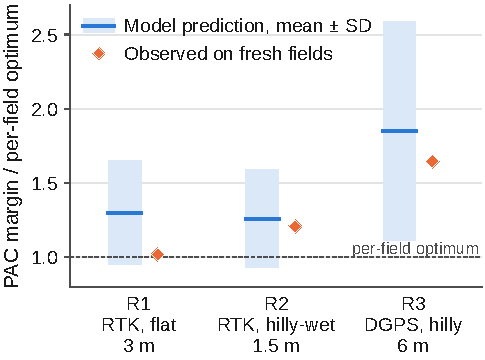
\includegraphics[width=\textwidth]{../../../figures/paper/fig_information_limit.pdf}
\renewcommand{\thefigure}{S3}\caption{Margin inflation under the ideal scale (Proposition A3 of the manuscript; post hoc). Blue line and box: prediction from the model alone (mean ± standard deviation over 2000 simulated calibrations, \(n=29\)); orange diamonds: observed on the 30 fresh E-low v2 fields of each configuration.}
\end{figure}

\begin{table}[!htbp]
\centering
\footnotesize
\renewcommand{\thetable}{S13}\caption{Theory pivot vs a ridge regression of \(\log\lambda^\star_f\) on six field features (log effective length, log area, log number of passes, mean slope, mean pass terrain feature, log lateral extent), trained on oracle targets on the E-low v1 pool (fields 80+, disjoint from the test fields) (post hoc). With oracle targets the feature model is slightly more accurate than the theory in R1 and R2; the theory is more accurate in R3.}
\begin{adjustbox}{max width=\textwidth}
\begin{tabular}{@{}ll>{\raggedright\arraybackslash}p{7.3em}>{\raggedright\arraybackslash}p{9.4em}>{\raggedright\arraybackslash}p{7.3em}>{\raggedright\arraybackslash}p{7.3em}>{\raggedright\arraybackslash}p{7.3em}@{}}
\toprule
\textbf{Regime} & \textbf{Train fields} & \textbf{Feature model train \(R^2\)} & \textbf{corr(log q, log λ*): theory / features / scale law} & \textbf{log-error sd: theory / features} & \textbf{Excess pp marginal: features / theory} & \textbf{Excess pp PAC: features / theory} \\
\midrule
R1 & 60 & 0.92 & 0.95 / 0.98 / 0.97 & 0.029 / 0.020 & −0.66 / −0.97 & +0.16 / +0.27 \\
R2 & 57 & 0.85 & 0.80 / 0.89 / 0.88 & 0.029 / 0.021 & +4.89 / +5.26 & +7.68 / +7.44 \\
R3 & 30 & 0.58 & 0.87 / 0.70 / 0.70 & 0.056 / 0.080 & −0.23 / −0.38 & +8.73 / +15.25 \\
\bottomrule
\end{tabular}
\end{adjustbox}
\end{table}

\begin{table}[!htbp]
\centering
\footnotesize
\renewcommand{\thetable}{S14}\caption{Standard deviation of \(\log(q/\lambda^\star)\) on the 30 v2 test fields (lower is better), mean over 40 random training subsets (one subset for the full pool). Post hoc; underlying data of Fig. S2.}
\begin{adjustbox}{max width=\textwidth}
\begin{tabular}{@{}>{\raggedright\arraybackslash}p{7.3em}>{\raggedright\arraybackslash}p{7.3em}>{\raggedright\arraybackslash}p{7.3em}>{\raggedright\arraybackslash}p{7.3em}>{\raggedright\arraybackslash}p{7.3em}@{}}
\toprule
\textbf{Regime (theory, zero data)} & \textbf{m training fields} & \textbf{features ← oracle targets} & \textbf{features ← one run} & \textbf{theory + features ← one run} \\
\midrule
R1 (0.029) & 5 & 0.044 & 0.355 & 0.177 \\
\textasciitilde{} & 10 & 0.030 & 0.173 & 0.107 \\
\textasciitilde{} & 20 & 0.023 & 0.141 & 0.098 \\
\textasciitilde{} & 30 & 0.022 & 0.130 & 0.105 \\
\textasciitilde{} & 60 & 0.020 & 0.095 & 0.091 \\
R2 (0.029) & 5 & 0.034 & 0.202 & 0.086 \\
\textasciitilde{} & 10 & 0.027 & 0.152 & 0.080 \\
\textasciitilde{} & 20 & 0.023 & 0.097 & 0.057 \\
\textasciitilde{} & 30 & 0.022 & 0.079 & 0.058 \\
\textasciitilde{} & 57 & 0.021 & 0.049 & 0.045 \\
R3 (0.056) & 5 & 0.123 & 0.406 & 0.220 \\
\textasciitilde{} & 10 & 0.094 & 0.324 & 0.216 \\
\textasciitilde{} & 20 & 0.083 & 0.246 & 0.169 \\
\textasciitilde{} & 30 & 0.080 & 0.206 & 0.146 \\
\bottomrule
\end{tabular}
\end{adjustbox}
\end{table}

\begin{figure}[!htbp]
\centering
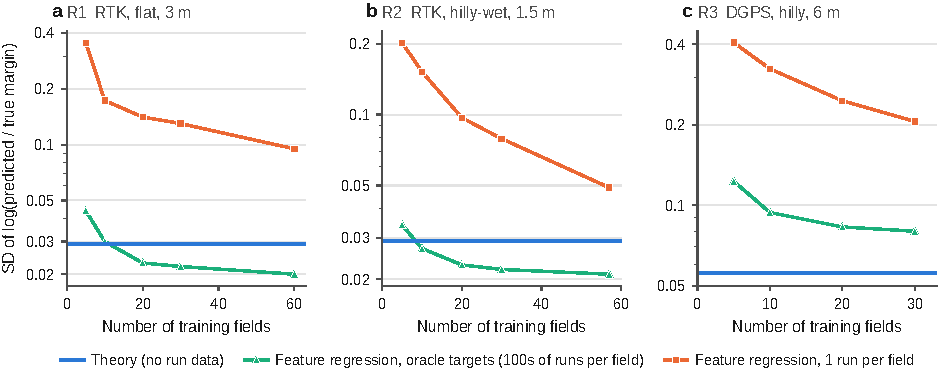
\includegraphics[width=\textwidth]{../../../figures/paper/fig_learning_curve.pdf}
\renewcommand{\thefigure}{S2}\caption{Learning curves of ridge regressions on field features (default penalty) against the zero-data model, standard deviation of log(prediction / \(\lambda^\star_f\)) on the 30 E-low v2 test fields (post hoc); Table S25 repeats the comparison with cross-validated learners.}
\end{figure}

\subsection*{D.6 E-low v3 (pre-registered; claims partially met)}
\addcontentsline{toc}{subsection}{D.6 E-low v3 (pre-registered; claims partially met)}

\begin{table}[!htbp]
\centering
\scriptsize
\renewcommand{\thetable}{S15}\caption{E-low v3, mixed fleet, registered reading (45 test fields from three machine configurations, 400 calibration subsets of \(n_\mathrm{cal}=25\) from a pool of 90). All methods valid by the registered criteria. Deployments below the lowest point of a field's curve grid (raw 485 and 69, scale law 648 and 106, CQR 284 and 113, CE-EVT-R 1 and 0, marginal and PAC, out of 400 × 45) have their coverage and overlap read at that lowest point (\(0.6\lambda^\star\)), which overstates both; Table S18 removes this.}
\begin{adjustbox}{max width=\textwidth}
\begin{tabular}{@{}>{\raggedright\arraybackslash}p{15.0em}>{\raggedright\arraybackslash}p{7.0em}ll>{\raggedright\arraybackslash}p{7.0em}>{\raggedright\arraybackslash}p{7.0em}ll>{\raggedright\arraybackslash}p{7.0em}@{}}
\toprule
\textbf{Method} & \textbf{Marginal: coverage mean} & \textbf{P(cov ≥ 0.9)} & \textbf{Excess pp} & \textbf{Matched-cov. excess pp} & \textbf{PAC: coverage mean} & \textbf{P(cov ≥ 0.9)} & \textbf{Excess pp} & \textbf{Matched-cov. excess pp} \\
\midrule
Raw pooling & 0.935 & 0.83 & +24.80 & +12.89 & 0.967 & 0.98 & +54.02 & +13.47 \\
Scale law & 0.935 & 0.84 & +33.97 & +17.22 & 0.967 & 0.97 & +66.95 & +17.07 \\
Spec × scale law & 0.930 & 0.69 & +13.18 & +10.68 & 0.973 & 0.95 & +20.05 & +9.97 \\
CQR (one-run trained) & 0.931 & 0.82 & +3.16 & +1.30 & 0.963 & 0.96 & +9.01 & +2.43 \\
\textbf{CE-EVT-R} & 0.918 & 0.55 & \textbf{+1.87} & \textbf{+0.73} & 0.958 & 0.86 & \textbf{+7.91} & +2.64 \\
CE-EVT-R-G (gate chose theory) & 0.916 & 0.54 & +1.73 & +0.98 & 0.960 & 0.88 & +8.50 & +3.52 \\
\bottomrule
\end{tabular}
\end{adjustbox}
\end{table}

\begin{table}[!htbp]
\centering
\scriptsize
\renewcommand{\thetable}{S16}\caption{E-low v3 registered comparisons (mean excess overlap over 400 calibration subsets; Holm over all 14 rows). C3: 5 of 8 comparisons met; the claim as registered (every comparator, both classes) is not met. C4: met in 1 of 6 cells.}
\begin{adjustbox}{max width=\textwidth}
\begin{tabular}{@{}ll>{\raggedright\arraybackslash}p{18.5em}lllll@{}}
\toprule
\textbf{Claim} & \textbf{Scenario / cell} & \textbf{Comparison} & \textbf{Ours pp} & \textbf{Comparator pp} & \textbf{Relative} & \textbf{Holm p} & \textbf{Outcome} \\
\midrule
C3 & mixed, marginal & vs raw & +1.87 & +24.80 & +92.5\% & 0.0000 & met \\
C3 & mixed, marginal & vs scale law & +1.87 & +33.97 & +94.5\% & 0.0000 & met \\
C3 & mixed, marginal & vs CQR & +1.87 & +3.16 & +40.9\% & 0.0029 & met \\
C3 & mixed, marginal & vs spec × scale law & +1.87 & +13.18 & +85.8\% & 0.1805 & not met \\
C3 & mixed, PAC & vs raw & +7.91 & +54.02 & +85.4\% & 0.0000 & met \\
C3 & mixed, PAC & vs scale law & +7.91 & +66.95 & +88.2\% & 0.0000 & met \\
C3 & mixed, PAC & vs CQR & +7.91 & +9.01 & +12.3\% & 0.0648 & not met \\
C3 & mixed, PAC & vs spec × scale law & +7.91 & +20.05 & +60.6\% & 0.9555 & not met \\
C4 & R1, marginal & gated (raw) vs best (CQR) & +0.17 & −0.29 & --- & 1.0000 & not met \\
C4 & R1, PAC & gated (scale law) vs best (scale law) & +0.39 & +0.37 & --- & 0.0003 & met \\
C4 & R2, marginal & gated (scale law) vs best (raw) & +6.12 & +5.63 & --- & 1.0000 & not met \\
C4 & R2, PAC & gated (theory) vs best (scale law) & +7.02 & +7.31 & --- & 0.1912 & not met \\
C4 & R3, marginal & gated (theory) vs best (CQR) & +3.93 & +1.09 & --- & 1.0000 & not met \\
C4 & R3, PAC & gated (raw) vs best (CQR) & +10.76 & +7.64 & --- & 1.0000 & not met \\
\bottomrule
\end{tabular}
\end{adjustbox}
\end{table}

\begin{table}[!htbp]
\centering
\scriptsize
\renewcommand{\thetable}{S17}\caption{E-low v3, same-regime cells (15 test fields each). Each method cell: mean excess pp / excess pp at matched coverage (mean coverage for marginal, fraction of subsets with coverage ≥ 0.9 for PAC). C5 for the mixed fleet: the gate chose the theory in both classes and the theory gained ≥ 10\% over raw (two hits); C5 total 5 of 8. C5 misses: R1 marginal and PAC, where the theory gained 201.2\% and 79.6\% over raw although the gate chose a classical pivot, and R3 marginal, where the gate chose the theory and the theory lost 61.4\% to raw.}
\begin{adjustbox}{max width=\textwidth}
\begin{tabular}{@{}ll>{\raggedright\arraybackslash}p{16.5em}ll>{\raggedright\arraybackslash}p{15.0em}>{\raggedright\arraybackslash}p{15.0em}ll@{}}
\toprule
\textbf{Regime} & \textbf{Class} & \textbf{Gate proxy excess pp (theory / raw / scale law) → choice} & \textbf{Raw} & \textbf{Scale law} & \textbf{CQR} & \textbf{CE-EVT-R} & \textbf{CE-EVT-R-G} & \textbf{C5} \\
\midrule
R1 & marginal & +1.60 / +1.52 / +1.52 → raw & +0.18 / +0.24 (0.896) & −0.02 / +0.08 (0.893) & −0.29 / +0.26 (0.861, invalid) & −0.18 / +0.15 (0.877, invalid) & +0.17 / +0.24 (0.896) & miss \\
R1 & PAC & +2.44 / +2.99 / +2.20 → scale law & +0.81 / +0.23 (0.97) & +0.37 / +0.06 (0.96) & +0.68 / +0.27 (0.85) & +0.17 / +0.07 (0.98) & +0.39 / +0.05 (0.98) & miss \\
R2 & marginal & +3.89 / +3.98 / +3.52 → scale law & +5.63 / +0.34 (0.967) & +6.14 / +0.29 (0.970) & +10.02 / +0.87 (0.983) & +5.39 / +0.27 (0.967) & +6.12 / +0.24 (0.970) & hit \\
R2 & PAC & +3.49 / +3.96 / +4.03 → theory & +7.95 / +0.24 (1.00) & +7.31 / +0.13 (1.00) & +22.11 / +0.84 (1.00) & +7.09 / +0.20 (1.00) & +7.02 / +0.21 (1.00) & hit \\
R3 & marginal & +4.14 / +4.83 / +4.64 → theory & +2.46 / +0.62 (0.924) & +2.35 / +0.56 (0.922) & +1.09 / +1.34 (0.897) & +3.97 / +1.64 (0.931) & +3.93 / +1.57 (0.931) & miss \\
R3 & PAC & +17.37 / +6.19 / +8.90 → raw & +10.99 / +1.22 (1.00) & +9.03 / +1.22 (1.00) & +7.64 / +1.65 (0.96) & +13.04 / +1.16 (0.97) & +10.76 / +1.44 (1.00) & hit \\
\bottomrule
\end{tabular}
\end{adjustbox}
\end{table}

\textbf{C3 details.} Against spec × scale law, the signed-rank test is driven by the per-field sign and rank of differences, so a large mean gain concentrated on part of the 45 test fields need not be significant (an interpretation; per-field differences are not tabulated). The CQR comparator already uses machine configuration as a feature; the classical scales that ignore the configuration are an order of magnitude worse, as the design probe predicted.

\textbf{C4 details.} The proxy difference between the theory and the best classical pivot was 0.08--0.50 pp in five of six cells. \textbf{Realised marginal coverage of CE-EVT-R in R1 was 0.877}, below the registered 0.89 threshold, so CE-EVT-R was formally invalid in that cell (as was CQR, 0.861), although coverage is averaged over 400 calibration subsets; these are all drawn from the same 30 fields with the same single historical run per field, so the luck of those runs is not averaged out (resolved by the resampling check, manuscript Section 6.4, Experiment B4).

\begin{table}[!htbp]
\centering
\footnotesize
\renewcommand{\thetable}{S18}\caption{E-low v3 re-read with margin curves extended down to \(0.25\lambda^\star\) (same seeds); only rows that differ from the registered reading are shown. No deployment falls below the curve grid any more. Every claim outcome is unchanged (C3 5 of 8, C4 1 of 6, C5 5 of 8); the C3 marginal comparison against CQR becomes +1.87 vs +3.15 pp (40.6\%, Holm p 0.0029) and the PAC comparison against CQR 12.2\% (Holm p 0.0648).}
\begin{adjustbox}{max width=\textwidth}
\begin{tabular}{@{}llllll>{\raggedright\arraybackslash}p{7.3em}@{}}
\toprule
\textbf{Scenario} & \textbf{Class} & \textbf{Method} & \textbf{Coverage mean} & \textbf{P(cov ≥ 0.9)} & \textbf{Excess pp} & \textbf{Matched-cov. excess pp} \\
\midrule
R3 & marginal & CQR & 0.896 & 0.72 & +1.08 & +1.40 \\
R3 & marginal & CE-EVT-R & 0.931 & 0.71 & +3.97 & +1.67 \\
R3 & PAC & CQR & 0.948 & 0.96 & +7.64 & +1.72 \\
R3 & PAC & CE-EVT-R & 0.971 & 0.97 & +13.04 & +1.21 \\
Mixed & marginal & Raw pooling & 0.933 & 0.83 & +24.78 & +15.54 \\
Mixed & marginal & Scale law & 0.931 & 0.84 & +33.94 & +20.55 \\
Mixed & marginal & CQR & 0.930 & 0.77 & +3.15 & +1.41 \\
Mixed & marginal & CE-EVT-R & 0.918 & 0.55 & +1.87 & +0.73 \\
Mixed & PAC & Raw pooling & 0.967 & 0.98 & +54.01 & +18.61 \\
Mixed & PAC & Scale law & 0.966 & 0.97 & +66.94 & +21.46 \\
Mixed & PAC & CQR & 0.962 & 0.96 & +9.01 & +2.54 \\
\bottomrule
\end{tabular}
\end{adjustbox}
\end{table}

\subsection*{D.7a Experiment B4 with the extended margin curves}
\addcontentsline{toc}{subsection}{D.7a Experiment B4 with the extended margin curves}

\begin{table}[!htbp]
\centering
\footnotesize
\renewcommand{\thetable}{S19a}\caption{Experiment B4, direct coverage check over 4000 replicates (pre-registered; random 25-field calibration split and redrawn historical run). Each cell: mean coverage / fraction of replicates with coverage ≥ 0.9 / mean excess overlap (pp, descriptive). Standard errors of mean coverage 0.0005--0.0008. Coverage and overlap are read from per-field margin curves extended to \(0.25\lambda^\star\). Every one of the 26 cells passes its criterion.}
\begin{adjustbox}{max width=\textwidth}
\begin{tabular}{@{}llllll@{}}
\toprule
\textbf{Scenario} & \textbf{Class} & \textbf{Raw pooling} & \textbf{Scale law} & \textbf{Spec × scale law} & \textbf{Theory (CE-EVT-R)} \\
\midrule
R1 & marginal & 0.9193 / 0.700 / +1.16 & 0.9205 / 0.707 / +0.92 & --- & 0.9194 / 0.689 / +0.92 \\
R1 & PAC & 0.9597 / 0.911 / +3.99 & 0.9604 / 0.911 / +3.75 & --- & 0.9607 / 0.917 / +3.77 \\
R2 & marginal & 0.9283 / 0.754 / +2.95 & 0.9282 / 0.767 / +2.90 & --- & 0.9286 / 0.759 / +3.06 \\
R2 & PAC & 0.9655 / 0.946 / +11.15 & 0.9652 / 0.949 / +10.63 & --- & 0.9641 / 0.935 / +10.56 \\
R3 & marginal & 0.9224 / 0.733 / +5.20 & 0.9214 / 0.717 / +4.74 & --- & 0.9211 / 0.717 / +5.06 \\
R3 & PAC & 0.9605 / 0.932 / +21.68 & 0.9595 / 0.926 / +21.04 & --- & 0.9603 / 0.930 / +21.45 \\
Mixed fleet & marginal & 0.9251 / 0.737 / +29.80 & 0.9244 / 0.747 / +37.18 & 0.9250 / 0.736 / +12.82 & 0.9243 / 0.747 / \textbf{+2.96} \\
Mixed fleet & PAC & 0.9612 / 0.934 / +61.97 & 0.9625 / 0.941 / +73.86 & 0.9629 / 0.928 / +23.21 & 0.9625 / 0.931 / \textbf{+14.69} \\
\bottomrule
\end{tabular}
\end{adjustbox}
\end{table}

\begin{figure}[!htbp]
\centering
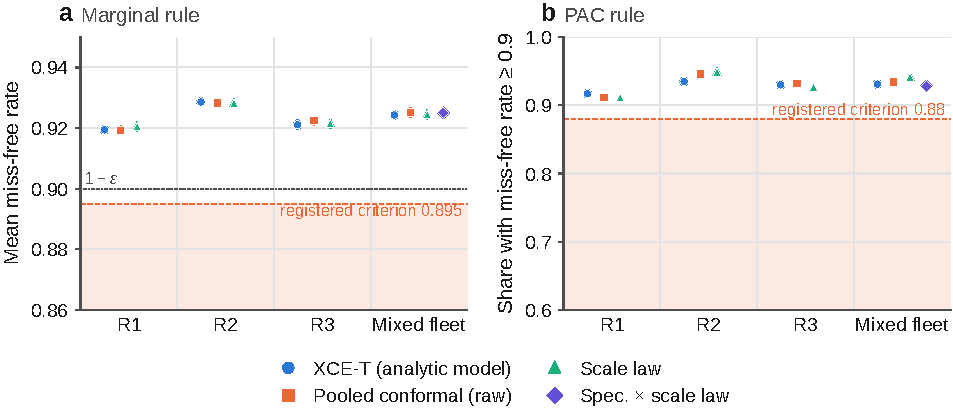
\includegraphics[width=\textwidth]{../../../figures/paper/fig_coverage_check.pdf}
\renewcommand{\thefigure}{S1}\caption{Experiment B4 (pre-registered; 4000 replicates per point). (a) Mean coverage of the marginal rule (bars: 95\% intervals); (b) share of replicates whose coverage reaches 0.9 under the PAC rule; dashed lines mark the registered criteria (0.895 and 0.88), the shaded region is the invalid side, and the dotted line in (a) marks \(1-\varepsilon=0.9\).}
\end{figure}

\subsection*{D.7 Resampling check with the registered curve grid}
\addcontentsline{toc}{subsection}{D.7 Resampling check with the registered curve grid}

\begin{table}[!htbp]
\centering
\footnotesize
\renewcommand{\thetable}{S19}\caption{Direct coverage check, registered reading with the \(0.6\lambda^\star\) curve-grid floor (mean coverage / fraction of replicates with coverage ≥ 0.9 / mean excess overlap, pp). All 26 cells pass; Table S19a uses the extended curves, which change only the raw and scale-law mixed-fleet cells (mean coverage by at most 0.0044, mean excess by at most 0.04 pp) and R3 raw marginal (0.9225 → 0.9224, +5.21 → +5.20 pp).}
\begin{adjustbox}{max width=\textwidth}
\begin{tabular}{@{}llllll@{}}
\toprule
\textbf{Scenario} & \textbf{Class} & \textbf{Raw pooling} & \textbf{Scale law} & \textbf{Spec × scale law} & \textbf{Theory (CE-EVT-R)} \\
\midrule
R1 & marginal & 0.9193 / 0.700 / +1.16 & 0.9205 / 0.707 / +0.92 & --- & 0.9194 / 0.689 / +0.92 \\
R1 & PAC & 0.9597 / 0.911 / +3.99 & 0.9604 / 0.911 / +3.75 & --- & 0.9607 / 0.917 / +3.77 \\
R2 & marginal & 0.9283 / 0.754 / +2.95 & 0.9282 / 0.767 / +2.90 & --- & 0.9286 / 0.759 / +3.06 \\
R2 & PAC & 0.9655 / 0.946 / +11.15 & 0.9652 / 0.949 / +10.63 & --- & 0.9641 / 0.935 / +10.56 \\
R3 & marginal & 0.9225 / 0.733 / +5.21 & 0.9214 / 0.717 / +4.74 & --- & 0.9211 / 0.717 / +5.06 \\
R3 & PAC & 0.9605 / 0.932 / +21.68 & 0.9595 / 0.926 / +21.04 & --- & 0.9603 / 0.930 / +21.45 \\
Mixed fleet & marginal & 0.9295 / 0.745 / +29.84 & 0.9283 / 0.750 / +37.21 & 0.9250 / 0.736 / +12.82 & 0.9243 / 0.747 / +2.96 \\
Mixed fleet & PAC & 0.9619 / 0.935 / +61.98 & 0.9631 / 0.942 / +73.86 & 0.9629 / 0.928 / +23.21 & 0.9625 / 0.931 / +14.69 \\
\bottomrule
\end{tabular}
\end{adjustbox}
\end{table}

\subsection*{D.8 Theory runtime}
\addcontentsline{toc}{subsection}{D.8 Theory runtime}

\begin{table}[!htbp]
\centering
\footnotesize
\renewcommand{\thetable}{S21}\caption{Single-core runtime of the theory predictor with 200 sampled operating conditions, three E-low v3 test fields per regime.}
\begin{adjustbox}{max width=\textwidth}
\begin{tabular}{@{}lll>{\raggedright\arraybackslash}p{7.3em}>{\raggedright\arraybackslash}p{7.3em}@{}}
\toprule
\textbf{Regime} & \textbf{Field (index)} & \textbf{Passes} & \textbf{Pass length (m)} & \textbf{Theory runtime (s)} \\
\midrule
R1 & 649 (5) & 16 & 2415 & 187 \\
R1 & 718 (10) & 10 & 1665 & 133 \\
R1 & 559 (15) & 90 & 3519 & 150 \\
R2 & 150 (5) & 73 & 5703 & 297 \\
R2 & 180 (10) & 83 & 5543 & 287 \\
R2 & 151 (15) & 41 & 5225 & 353 \\
R3 & 119 (5) & 18 & 458 & 23 \\
R3 & 74 (10) & 23 & 1016 & 51 \\
R3 & 215 (15) & 7 & 324 & 16 \\
\bottomrule
\end{tabular}
\end{adjustbox}
\end{table}

\subsection*{D.10 Revision experiments}
\addcontentsline{toc}{subsection}{D.10 Revision experiments}

\begin{table}[!htbp]
\centering
\footnotesize
\renewcommand{\thetable}{S23}\caption{Experiment A1: every CE / CE+ row on every planner--controller stack (descriptive). A correctly calibrated marginal method meets the per-field test on about 85\% of fields and a PAC method on about 99\% (Proposition A4). The one failure is CE+ on follow-previous-pass guidance in R2 (P 0.850, meet 0.70).}
\begin{adjustbox}{max width=\textwidth}
\begin{tabular}{@{}l>{\raggedright\arraybackslash}p{20.8em}ll@{}}
\toprule
\textbf{Config.} & \textbf{System} & \textbf{P(no miss)} & \textbf{Meet rate} \\
\midrule
R1 & BCD + LQR-I + CE (ours) & 0.937 & 1.00 \\
R1 & BCD + LQR-I + CE+ (ours, v8) & 0.903 & 0.93 \\
R1 & BCD + LQR-I + CE+ PAC (ours, v8) & 0.941 & 1.00 \\
R1 & BCD + LQR-I + CE-q (ours, Thm 2) & 0.904 & 0.87 \\
R1 & BCD + Lenain ctrl + CE (ours) & 0.934 & 1.00 \\
R1 & BCD + Lenain ctrl + CE+ (ours, v8) & 0.909 & 0.93 \\
R1 & BCD + Lenain ctrl + CE+ PAC (ours, v8) & 0.942 & 1.00 \\
R1 & BCD + Lenain ctrl + CE-q (ours, Thm 2) & 0.904 & 0.93 \\
R1 & BCD + offset-free MPC + CE (ours) & 0.932 & 1.00 \\
R1 & BCD + offset-free MPC + CE+ (ours, v8) & 0.902 & 0.80 \\
R1 & BCD + offset-free MPC + CE+ PAC (ours, v8) & 0.940 & 1.00 \\
R1 & BCD + offset-free MPC + CE-q (ours, Thm 2) & 0.907 & 0.97 \\
R1 & Fields2Cover + LQR-I + CE (ours) & 0.941 & 1.00 \\
R1 & Fields2Cover + LQR-I + CE+ (ours, v8) & 0.914 & 0.97 \\
R1 & Fields2Cover + LQR-I + CE+ PAC (ours, v8) & 0.947 & 1.00 \\
R1 & Fields2Cover + LQR-I + CE-q (ours, Thm 2) & 0.897 & 0.83 \\
R1 & Follow-previous-pass + LQR-I + CE (ours) & 0.938 & 1.00 \\
R1 & Follow-previous-pass + LQR-I + CE+ (ours, v8) & 0.907 & 0.93 \\
R1 & Follow-previous-pass + LQR-I + CE+ PAC (ours, v8) & 0.942 & 1.00 \\
R1 & Follow-previous-pass + Lenain ctrl + CE+ (ours, v8) & 0.911 & 0.93 \\
R1 & Follow-previous-pass + Lenain ctrl + CE+ PAC (ours, v8) & 0.941 & 1.00 \\
R1 & Hameed 3D + LQR-I + CE (ours) & 0.941 & 1.00 \\
R1 & Hameed 3D + LQR-I + CE+ (ours, v8) & 0.904 & 0.93 \\
R1 & Hameed 3D + LQR-I + CE+ PAC (ours, v8) & 0.944 & 1.00 \\
R2 & BCD + LQR-I + CE (ours) & 0.944 & 1.00 \\
R2 & BCD + LQR-I + CE+ (ours, v8) & 0.911 & 0.90 \\
R2 & BCD + LQR-I + CE+ PAC (ours, v8) & 0.944 & 1.00 \\
R2 & BCD + LQR-I + CE-q (ours, Thm 2) & 0.905 & 0.87 \\
R2 & BCD + Lenain ctrl + CE (ours) & 0.946 & 1.00 \\
R2 & BCD + Lenain ctrl + CE+ (ours, v8) & 0.914 & 0.93 \\
R2 & BCD + Lenain ctrl + CE+ PAC (ours, v8) & 0.948 & 1.00 \\
R2 & BCD + Lenain ctrl + CE-q (ours, Thm 2) & 0.894 & 0.80 \\
R2 & BCD + offset-free MPC + CE (ours) & 0.944 & 1.00 \\
R2 & BCD + offset-free MPC + CE+ (ours, v8) & 0.909 & 0.93 \\
R2 & BCD + offset-free MPC + CE+ PAC (ours, v8) & 0.946 & 1.00 \\
R2 & BCD + offset-free MPC + CE-q (ours, Thm 2) & 0.911 & 0.90 \\
R2 & Fields2Cover + LQR-I + CE (ours) & 0.938 & 1.00 \\
R2 & Fields2Cover + LQR-I + CE+ (ours, v8) & 0.905 & 0.90 \\
R2 & Fields2Cover + LQR-I + CE+ PAC (ours, v8) & 0.946 & 1.00 \\
R2 & Fields2Cover + LQR-I + CE-q (ours, Thm 2) & 0.894 & 0.83 \\
R2 & Follow-previous-pass + LQR-I + CE (ours) & 0.945 & 0.87 \\
R2 & Follow-previous-pass + LQR-I + CE+ (ours, v8) & 0.850 & 0.70 \\
R2 & Follow-previous-pass + LQR-I + CE+ PAC (ours, v8) & 0.941 & 0.87 \\
R2 & Follow-previous-pass + Lenain ctrl + CE+ (ours, v8) & 0.886 & 0.80 \\
R2 & Follow-previous-pass + Lenain ctrl + CE+ PAC (ours, v8) & 0.933 & 0.90 \\
R2 & Hameed 3D + LQR-I + CE (ours) & 0.942 & 1.00 \\
R2 & Hameed 3D + LQR-I + CE+ (ours, v8) & 0.911 & 0.87 \\
R2 & Hameed 3D + LQR-I + CE+ PAC (ours, v8) & 0.942 & 0.97 \\
R3 & BCD + LQR-I + CE (ours) & 0.928 & 0.97 \\
R3 & BCD + LQR-I + CE+ (ours, v8) & 0.896 & 0.90 \\
R3 & BCD + LQR-I + CE+ PAC (ours, v8) & 0.933 & 1.00 \\
R3 & BCD + LQR-I + CE-q (ours, Thm 2) & 0.903 & 0.83 \\
R3 & BCD + Lenain ctrl + CE (ours) & 0.927 & 1.00 \\
R3 & BCD + Lenain ctrl + CE+ (ours, v8) & 0.903 & 0.83 \\
R3 & BCD + Lenain ctrl + CE+ PAC (ours, v8) & 0.941 & 0.97 \\
R3 & BCD + Lenain ctrl + CE-q (ours, Thm 2) & 0.897 & 0.77 \\
R3 & BCD + offset-free MPC + CE (ours) & 0.926 & 1.00 \\
R3 & BCD + offset-free MPC + CE+ (ours, v8) & 0.891 & 0.77 \\
R3 & BCD + offset-free MPC + CE+ PAC (ours, v8) & 0.931 & 1.00 \\
R3 & BCD + offset-free MPC + CE-q (ours, Thm 2) & 0.902 & 0.87 \\
R3 & Fields2Cover + LQR-I + CE (ours) & 0.928 & 1.00 \\
R3 & Fields2Cover + LQR-I + CE+ (ours, v8) & 0.903 & 0.90 \\
R3 & Fields2Cover + LQR-I + CE+ PAC (ours, v8) & 0.941 & 1.00 \\
R3 & Fields2Cover + LQR-I + CE-q (ours, Thm 2) & 0.915 & 0.90 \\
R3 & Follow-previous-pass + LQR-I + CE (ours) & 0.930 & 1.00 \\
R3 & Follow-previous-pass + LQR-I + CE+ (ours, v8) & 0.895 & 0.87 \\
R3 & Follow-previous-pass + LQR-I + CE+ PAC (ours, v8) & 0.941 & 1.00 \\
R3 & Follow-previous-pass + Lenain ctrl + CE+ (ours, v8) & 0.902 & 0.93 \\
R3 & Follow-previous-pass + Lenain ctrl + CE+ PAC (ours, v8) & 0.940 & 0.97 \\
R3 & Hameed 3D + LQR-I + CE (ours) & 0.924 & 1.00 \\
R3 & Hameed 3D + LQR-I + CE+ (ours, v8) & 0.900 & 0.83 \\
R3 & Hameed 3D + LQR-I + CE+ PAC (ours, v8) & 0.937 & 1.00 \\
\bottomrule
\end{tabular}
\end{adjustbox}
\end{table}

\begin{table}[!htbp]
\centering
\footnotesize
\renewcommand{\thetable}{S24}\caption{Experiment A2 (pre-registered): CE-q with \(n\) runs from 200-run banks, 45 fields per configuration, 2000 replicates per field. Exact marginal targets \(k_\star/(n+1)\): 0.900, 0.938, 0.913, 0.902, 0.901 for \(n=9,15,22,40,100\).}
\begin{adjustbox}{max width=\textwidth}
\begin{tabular}{@{}ll>{\raggedright\arraybackslash}p{15.6em}lll@{}}
\toprule
\textbf{Config.} & \textbf{\(n\)} & \textbf{Rule} & \textbf{Mean coverage} & \textbf{Fraction ≥ 0.9} & \textbf{Excess pp} \\
\midrule
R1 & 9 & marginal & 0.8984 & 0.603 & +1.29 \\
R1 & 15 & marginal & 0.9359 & 0.782 & +2.41 \\
R1 & 22 & marginal & 0.9103 & 0.643 & +0.68 \\
R1 & 22 & PAC & 0.9555 & 0.890 & +3.37 \\
R1 & 40 & marginal & 0.8988 & 0.551 & +0.22 \\
R1 & 40 & PAC & 0.9497 & 0.902 & +1.77 \\
R1 & 100 & marginal & 0.8960 & 0.494 & +0.05 \\
R1 & 100 & PAC & 0.9381 & 0.915 & +1.05 \\
R1 & --- & farmer-tuned (\(\lambda\) = 0.120 m) & 0.8857 & 0.511 & +0.12 \\
R1 & --- & vendor 2x p2p (\(\lambda\) = 0.025 m) & 0.0000 & 0.000 & -6.81 \\
R2 & 9 & marginal & 0.9058 & 0.637 & +4.02 \\
R2 & 15 & marginal & 0.9426 & 0.816 & +7.31 \\
R2 & 22 & marginal & 0.9192 & 0.693 & +2.30 \\
R2 & 22 & PAC & 0.9606 & 0.916 & +10.03 \\
R2 & 40 & marginal & 0.9098 & 0.632 & +0.99 \\
R2 & 40 & PAC & 0.9560 & 0.933 & +5.42 \\
R2 & 100 & marginal & 0.9086 & 0.639 & +0.56 \\
R2 & 100 & PAC & 0.9469 & 0.951 & +3.20 \\
R2 & --- & farmer-tuned (\(\lambda\) = 0.140 m) & 0.8463 & 0.022 & -1.93 \\
R2 & --- & vendor 2x p2p (\(\lambda\) = 0.025 m) & 0.0000 & 0.000 & -19.62 \\
R3 & 9 & marginal & 0.8997 & 0.613 & +8.29 \\
R3 & 15 & marginal & 0.9362 & 0.790 & +13.76 \\
R3 & 22 & marginal & 0.9117 & 0.659 & +3.97 \\
R3 & 22 & PAC & 0.9551 & 0.896 & +18.70 \\
R3 & 40 & marginal & 0.9006 & 0.572 & +1.39 \\
R3 & 40 & PAC & 0.9498 & 0.910 & +9.65 \\
R3 & 100 & marginal & 0.8982 & 0.535 & +0.57 \\
R3 & 100 & PAC & 0.9382 & 0.917 & +4.32 \\
R3 & --- & farmer-tuned (\(\lambda\) = 0.350 m) & 0.8447 & 0.200 & -1.69 \\
R3 & --- & vendor 2x p2p (\(\lambda\) = 0.200 m) & 0.4325 & 0.000 & -7.52 \\
\bottomrule
\end{tabular}
\end{adjustbox}
\end{table}

\begin{table}[!htbp]
\centering
\footnotesize
\renewcommand{\thetable}{S25}\caption{Experiment B6 (descriptive, post hoc): standard deviation of log(prediction / \(\lambda^\star_f\)) on the 30 E-low v2 test fields, mean over 20 random training subsets (one for the full pool), trained on the disjoint E-low v1 pool. Penalties and learning rates chosen by 5-fold cross-validation on the training fields.}
\begin{adjustbox}{max width=\textwidth}
\begin{tabular}{@{}>{\raggedright\arraybackslash}p{16.1em}l>{\raggedright\arraybackslash}p{15.1em}>{\raggedright\arraybackslash}p{15.1em}>{\raggedright\arraybackslash}p{15.1em}>{\raggedright\arraybackslash}p{15.1em}>{\raggedright\arraybackslash}p{15.1em}@{}}
\toprule
\textbf{Config.} & \textbf{Training fields} & \textbf{Ridge (CV), one run} & \textbf{Gradient boosting (CV), one run} & \textbf{Model + ridge correction (CV), one run} & \textbf{Ridge (CV), oracle targets} & \textbf{Gradient boosting, oracle targets} \\
\midrule
R1 (model 0.029; MC twin 0.025) & 10 / 20 / 30 / 60 & 0.193 / 0.128 / 0.078 / 0.070 & 0.153 / 0.119 / 0.124 / 0.109 & 0.129 / 0.105 / 0.072 / 0.063 & 0.029 / 0.025 / 0.023 / 0.021 & 0.044 / 0.036 / 0.032 / 0.034 \\
R2 (model 0.029; MC twin 0.026) & 10 / 20 / 30 / 57 & 0.054 / 0.048 / 0.048 / 0.043 & 0.087 / 0.088 / 0.078 / 0.049 & 0.045 / 0.037 / 0.036 / 0.029 & 0.032 / 0.023 / 0.022 / 0.021 & 0.031 / 0.028 / 0.027 / 0.025 \\
R3 (model 0.056; MC twin 0.047) & 10 / 20 / 30 & 0.281 / 0.178 / 0.148 & 0.218 / 0.264 / 0.190 & 0.248 / 0.159 / 0.124 & 0.106 / 0.082 / 0.079 & 0.086 / 0.075 / 0.072 \\
\bottomrule
\end{tabular}
\end{adjustbox}
\end{table}

\begin{table}[!htbp]
\centering
\footnotesize
\renewcommand{\thetable}{S28}\caption{Experiment C2 (pre-registered): headland laps, 45 fields per configuration (oracle columns: fields with both curves, 41--42). CE-q columns: mean coverage (marginal) and fraction of replicates with coverage ≥ 0.9 (PAC).}
\begin{adjustbox}{max width=\textwidth}
\begin{tabular}{@{}l>{\raggedright\arraybackslash}p{7.3em}>{\raggedright\arraybackslash}p{7.3em}>{\raggedright\arraybackslash}p{7.3em}>{\raggedright\arraybackslash}p{7.3em}>{\raggedright\arraybackslash}p{10.9em}@{}}
\toprule
\textbf{Config.} & \textbf{Binding term is a boundary term: hard edge / laps} & \textbf{0.9 score quantile: hard edge / laps (m)} & \textbf{Oracle margin: hard edge / laps (m)} & \textbf{Overlap at oracle: hard edge / laps (\%)} & \textbf{CE-q with laps: \(n=9\) marginal / \(n=100\) marginal / \(n=22\) PAC} \\
\midrule
R1 & 0.010 / 0.001 & 0.121 / 0.120 & 0.121 / 0.121 & 8.89 / 8.93 & 0.897 / 0.898 / 0.885 \\
R2 & 0.008 / 0.001 & 0.150 / 0.149 & 0.149 / 0.149 & 24.91 / 24.87 & 0.899 / 0.899 / 0.902 \\
R3 & 0.100 / 0.019 & 0.388 / 0.366 & 0.391 / 0.366 & 15.12 / 14.01 & 0.902 / 0.901 / 0.907 \\
\bottomrule
\end{tabular}
\end{adjustbox}
\end{table}

\textbf{Table S26. Experiment B5 (pre-registered), full output.} Columns: pivot, rule, overall coverage (marginal: mean; PAC: fraction of replicates with coverage ≥ 0.9), validity criterion, refusal rate, coverage per configuration (R1, R2, R3), mean excess overlap over deployed fields and with the cap for refused fields (pp).

\begin{Verbatim}[fontsize=\tiny,breaklines]
== mixed fleet, 135 fields, n_cal = 25, 4000 replicates
  pivot              class    coverage valid refuse   cov R1   cov R2   cov R3 excess(dep) excess(cap)
  raw                marginal   0.9244  PASS  0.000    0.999    0.998    0.779      +29.19      +29.19
  spec x scale law   marginal   0.9253  PASS  0.000    0.944    0.840    0.993      +12.95      +12.95
  theory             marginal   0.9237  PASS  0.000    0.931    0.936    0.904       +2.89       +2.89
  theory+edges       marginal   0.9251  PASS  0.000    0.931    0.936    0.908       +3.05       +3.05
  Mondrian           marginal   0.9601  PASS  0.560    0.958    0.960    0.957       +5.83     +128.30
  per-config scale   marginal   0.9129  PASS  0.000    0.939    0.958    0.842       +4.57       +4.57
  CQR                marginal   0.9231  PASS  0.000    0.961    0.942    0.866       +4.09       +4.09
  MC twin            marginal   0.9222  PASS  0.000    0.924    0.929    0.913       +2.68       +2.68
  raw                PAC         0.926  PASS  0.000    1.000    1.000    0.582      +63.97      +63.97
  spec x scale law   PAC         0.926  PASS  0.000    0.966    0.701    1.000      +23.09      +23.09
  theory             PAC         0.933  PASS  0.000    0.943    0.948    0.860      +14.56      +14.56
  theory+edges       PAC         0.932  PASS  0.000    0.939    0.948    0.882      +14.08      +14.08
  Mondrian           PAC         1.000  PASS  1.000    1.000    1.000    1.000        +nan     +224.86
  per-config scale   PAC         0.892  PASS  0.000    0.928    0.971    0.670      +19.94      +19.94
  CQR                PAC         0.929  PASS  0.000    0.987    0.958    0.717      +18.86      +18.86
  MC twin            PAC         0.931  PASS  0.000    0.929    0.942    0.907      +13.76      +13.76

== mixed fleet, 135 fields, n_cal = 60, 4000 replicates
  pivot              class    coverage valid refuse   cov R1   cov R2   cov R3 excess(dep) excess(cap)
  raw                marginal   0.9036  PASS  0.000    0.999    0.998    0.718      +17.12      +17.12
  spec x scale law   marginal   0.9040  PASS  0.000    0.929    0.794    0.992       +9.93       +9.93
  theory             marginal   0.9029  PASS  0.000    0.909    0.915    0.885       +0.57       +0.57
  theory+edges       marginal   0.9029  PASS  0.000    0.907    0.913    0.889       +0.57       +0.57
  Mondrian           marginal   0.9212  PASS  0.000    0.918    0.926    0.918       +4.35       +4.35
  per-config scale   marginal   0.8960  PASS  0.000    0.923    0.949    0.816       +1.29       +1.29
  CQR                marginal   0.9044  PASS  0.000    0.950    0.925    0.838       +1.20       +1.20
  MC twin            marginal   0.9025  PASS  0.000    0.902    0.909    0.897       +0.55       +0.55
  raw                PAC         0.942  PASS  0.000    1.000    1.000    0.333      +37.98      +37.98
  spec x scale law   PAC         0.944  PASS  0.000    0.988    0.560    1.000      +14.98      +14.98
  theory             PAC         0.948  PASS  0.000    0.962    0.972    0.834       +4.37       +4.37
  theory+edges       PAC         0.947  PASS  0.000    0.956    0.966    0.864       +4.40       +4.40
  Mondrian           PAC         1.000  PASS  0.743    0.972    0.975    0.976      +12.19     +170.36
  per-config scale   PAC         0.934  PASS  0.000    0.967    0.993    0.500       +6.42       +6.42
  CQR                PAC         0.955  PASS  0.000    0.998    0.980    0.559       +6.19       +6.19
  MC twin            PAC         0.946  PASS  0.000    0.942    0.957    0.914       +4.19       +4.19
\end{Verbatim}

\textbf{Table S27. Experiment C1 (pre-registered), outcome of the registered predictions.} P4.1 (overall validity of every non-refusing pivot in every variant): met in T2--T6; not met in T1 at 60 calibration fields (marginal mean coverage 0.892--0.895 against 0.895), where the deployed margin exceeded the reference margin on most RTK fields. P4.2 (model log-error standard deviation below 0.15 in every configuration and variant): not met in T1 (R1 0.210), T3 (R3 0.730) and T6 (R1 0.263, R2 0.158). P4.3 (mixed fleet, 25 calibration fields, marginal: model pivot excess below half of raw pooling and below the specification scale): met in T2, T4 and T5; not met in T1 (17.03 vs 25.87 pp for raw pooling), T3 (20.84 vs 15.60 pp for the specification scale) and T6 (63.65 vs 37.69 pp). P4.4 (CE-q marginal mean coverage ≥ 0.895 in every variant): not met in T1 with 100 runs (R1 0.893, R2 0.891); met elsewhere. Full output (\texttt{results/revision/rv4\_mismatch.txt}):

\begin{Verbatim}[fontsize=\tiny,breaklines]
**T1 wet patches: 135 fields**
  R1 accuracy theory       : log(q/q_truth) mean -0.733 sd 0.210
  R1 accuracy theory+edges : log(q/q_truth) mean -0.733 sd 0.210
  R1 accuracy MC twin      : log(q/q_truth) mean -0.739 sd 0.213
  R1 fields without a feasible truth oracle: 0/45
  R2 accuracy theory       : log(q/q_truth) mean -0.720 sd 0.129
  R2 accuracy theory+edges : log(q/q_truth) mean -0.720 sd 0.129
  R2 accuracy MC twin      : log(q/q_truth) mean -0.723 sd 0.129
  R2 fields without a feasible truth oracle: 0/45
  R3 accuracy theory       : log(q/q_truth) mean -0.082 sd 0.085
  R3 accuracy theory+edges : log(q/q_truth) mean -0.066 sd 0.089
  R3 accuracy MC twin      : log(q/q_truth) mean -0.039 sd 0.062
  R3 fields without a feasible truth oracle: 0/45

== T1 wet patches: mixed fleet, 135 feasible fields, n_cal = 25, 2000 replicates
  pivot              class    coverage valid refuse   cov R1   cov R2   cov R3 excess(dep) excess(cap)
  raw                marginal   0.9230  PASS  0.000    0.953    0.951    0.866      +25.87      +25.87
  spec x scale law   marginal   0.9183  PASS  0.000    0.899    0.858    1.000      +64.61      +64.61
  theory+edges       marginal   0.9191  PASS  0.000    0.877    0.896    0.986      +17.03      +17.03
  Mondrian           marginal   0.9586  PASS  0.557    0.955    0.956    0.958      +26.86     +135.36
  MC twin            marginal   0.9182  PASS  0.000    0.875    0.894    0.987      +16.63      +16.63
  raw                PAC         0.903  PASS  0.000    0.998    0.962    0.779      +64.20      +64.20
  spec x scale law   PAC         0.914  PASS  0.000    0.871    0.732    1.000     +104.71     +104.71
  theory+edges       PAC         0.905  PASS  0.000    0.809    0.827    1.000      +58.83      +58.83
  Mondrian           PAC         1.000  PASS  1.000    1.000    1.000    1.000        +nan     +221.97
  MC twin            PAC         0.903  PASS  0.000    0.802    0.832    1.000      +60.69      +60.69

== T1 wet patches: mixed fleet, 135 feasible fields, n_cal = 60, 2000 replicates
  pivot              class    coverage valid refuse   cov R1   cov R2   cov R3 excess(dep) excess(cap)
  raw                marginal   0.8941  FAIL  0.000    0.939    0.922    0.823       +7.81       +7.81
  spec x scale law   marginal   0.8924  FAIL  0.000    0.871    0.808    0.999      +45.53      +45.53
  theory+edges       marginal   0.8948  FAIL  0.000    0.846    0.857    0.982       +1.79       +1.79
  Mondrian           marginal   0.9197  PASS  0.000    0.915    0.924    0.917      +23.49      +23.49
  MC twin            marginal   0.8940  FAIL  0.000    0.844    0.855    0.983       +1.77       +1.77
  raw                PAC         0.920  PASS  0.000    0.999    0.976    0.707      +40.69      +40.69
  spec x scale law   PAC         0.915  PASS  0.000    0.827    0.559    1.000      +82.04      +82.04
  theory+edges       PAC         0.908  PASS  0.000    0.728    0.782    1.000      +28.39      +28.39
  Mondrian           PAC         0.999  PASS  0.747    0.974    0.965    0.972      +56.99     +180.06
  MC twin            PAC         0.905  PASS  0.000    0.719    0.771    1.000      +27.67      +27.67

== T1 wet patches: target-field CE-q: target-field CE-q from n runs of the field's bank (500 replicates per field); coverage = mean P(no miss) / fraction of cells >= 0.9; excess pp
  R1 (45 fields)
    n=  9 marginal coverage 0.8959 / 0.586  excess +13.06
    n= 15 marginal coverage 0.9336 / 0.761  excess +22.88
    n= 22 marginal coverage 0.9063 / 0.609  excess  +5.28
    n= 22 PAC      coverage 0.9538 / 0.871  excess +32.61
    n= 40 marginal coverage 0.8948 / 0.513  excess  +0.58
    n= 40 PAC      coverage 0.9473 / 0.877  excess +15.67
    n=100 marginal coverage 0.8926 / 0.463  excess  -0.81
    n=100 PAC      coverage 0.9344 / 0.857  excess  +5.54
    farmer-tuned lam 0.120: coverage 0.3275 / 0.000  excess -14.62
    vendor 2x p2p lam 0.025: coverage 0.0002 / 0.000  excess -19.07
  R2 (45 fields)
    n=  9 marginal coverage 0.9011 / 0.562  excess +42.27
    n= 15 marginal coverage 0.9437 / 0.747  excess +73.14
    n= 22 marginal coverage 0.9142 / 0.586  excess +29.42
    n= 22 PAC      coverage 0.9665 / 0.864  excess +98.85
    n= 40 marginal coverage 0.8982 / 0.476  excess  +8.49
    n= 40 PAC      coverage 0.9634 / 0.870  excess +73.33
    n=100 marginal coverage 0.8909 / 0.380  excess  -0.96
    n=100 PAC      coverage 0.9523 / 0.865  excess +38.49
    farmer-tuned lam 0.140: coverage 0.2314 / 0.000  excess -56.18
    vendor 2x p2p lam 0.025: coverage 0.0004 / 0.000  excess -67.49
  R3 (45 fields)
    n=  9 marginal coverage 0.8968 / 0.593  excess  +8.01
    n= 15 marginal coverage 0.9349 / 0.778  excess +13.54
    n= 22 marginal coverage 0.9099 / 0.632  excess  +3.49
    n= 22 PAC      coverage 0.9545 / 0.886  excess +18.71
    n= 40 marginal coverage 0.8990 / 0.538  excess  +1.00
    n= 40 PAC      coverage 0.9488 / 0.901  excess  +8.92
    n=100 marginal coverage 0.8972 / 0.489  excess  +0.19
    n=100 PAC      coverage 0.9383 / 0.912  excess  +3.97
    farmer-tuned lam 0.350: coverage 0.8188 / 0.111  excess  -2.83
    vendor 2x p2p lam 0.200: coverage 0.3676 / 0.000  excess  -8.66

**T2 trailed implement: 135 fields**
  R1 accuracy theory       : log(q/q_truth) mean +0.418 sd 0.042
  R1 accuracy theory+edges : log(q/q_truth) mean +0.418 sd 0.042
  R1 accuracy MC twin      : log(q/q_truth) mean +0.413 sd 0.042
  R1 fields without a feasible truth oracle: 0/45
  R2 accuracy theory       : log(q/q_truth) mean +0.434 sd 0.059
  R2 accuracy theory+edges : log(q/q_truth) mean +0.434 sd 0.059
  R2 accuracy MC twin      : log(q/q_truth) mean +0.431 sd 0.059
  R2 fields without a feasible truth oracle: 0/45
  R3 accuracy theory       : log(q/q_truth) mean +0.024 sd 0.099
  R3 accuracy theory+edges : log(q/q_truth) mean +0.040 sd 0.105
  R3 accuracy MC twin      : log(q/q_truth) mean +0.067 sd 0.080
  R3 fields without a feasible truth oracle: 0/45

== T2 trailed implement: mixed fleet, 135 feasible fields, n_cal = 25, 2000 replicates
  pivot              class    coverage valid refuse   cov R1   cov R2   cov R3 excess(dep) excess(cap)
  raw                marginal   0.9239  PASS  0.000    0.998    0.999    0.777      +28.46      +28.46
  spec x scale law   marginal   0.9227  PASS  0.000    0.940    0.850    0.978       +5.68       +5.68
  theory+edges       marginal   0.9239  PASS  0.000    0.964    0.970    0.838       +3.15       +3.15
  Mondrian           marginal   0.9603  PASS  0.557    0.959    0.957    0.959       +5.79     +127.67
  MC twin            marginal   0.9253  PASS  0.000    0.961    0.968    0.847       +2.90       +2.90
  raw                PAC         0.939  PASS  0.000    1.000    1.000    0.582      +58.38      +58.38
  spec x scale law   PAC         0.916  PASS  0.000    0.967    0.706    1.000      +13.11      +13.11
  theory+edges       PAC         0.937  PASS  0.000    0.993    0.994    0.663      +14.59      +14.59
  Mondrian           PAC         1.000  PASS  1.000    1.000    1.000    1.000        +nan     +224.72
  MC twin            PAC         0.945  PASS  0.000    0.993    0.995    0.652      +12.34      +12.34

== T2 trailed implement: mixed fleet, 135 feasible fields, n_cal = 60, 2000 replicates
  pivot              class    coverage valid refuse   cov R1   cov R2   cov R3 excess(dep) excess(cap)
  raw                marginal   0.9028  PASS  0.000    0.998    0.999    0.716      +17.86      +17.86
  spec x scale law   marginal   0.9023  PASS  0.000    0.925    0.808    0.975       +3.93       +3.93
  theory+edges       marginal   0.9034  PASS  0.000    0.953    0.961    0.797       +0.65       +0.65
  Mondrian           marginal   0.9215  PASS  0.000    0.917    0.924    0.921       +3.81       +3.81
  MC twin            marginal   0.9034  PASS  0.000    0.948    0.957    0.805       +0.52       +0.52
  raw                PAC         0.945  PASS  0.000    1.000    1.000    0.352      +36.60      +36.60
  spec x scale law   PAC         0.941  PASS  0.000    0.990    0.594    1.000       +6.80       +6.80
  theory+edges       PAC         0.940  PASS  0.000    0.999    1.000    0.458       +4.59       +4.59
  Mondrian           PAC         1.000  PASS  0.747    0.972    0.975    0.974       +9.43     +170.35
  MC twin            PAC         0.948  PASS  0.000    0.998    0.999    0.463       +4.36       +4.36

== T2 trailed implement: target-field CE-q: target-field CE-q from n runs of the field's bank (500 replicates per field); coverage = mean P(no miss) / fraction of cells >= 0.9; excess pp
  R1 (45 fields)
    n=  9 marginal coverage 0.8989 / 0.610  excess  +0.90
    n= 15 marginal coverage 0.9354 / 0.787  excess  +1.63
    n= 22 marginal coverage 0.9111 / 0.655  excess  +0.42
    n= 22 PAC      coverage 0.9548 / 0.892  excess  +2.32
    n= 40 marginal coverage 0.9010 / 0.581  excess  +0.11
    n= 40 PAC      coverage 0.9489 / 0.895  excess  +1.14
    n=100 marginal coverage 0.8998 / 0.571  excess  +0.03
    n=100 PAC      coverage 0.9378 / 0.889  excess  +0.55
    farmer-tuned lam 0.120: coverage 0.9872 / 1.000  excess  +3.37
    vendor 2x p2p lam 0.025: coverage 0.0026 / 0.000  excess  -3.86
  R2 (45 fields)
    n=  9 marginal coverage 0.9035 / 0.614  excess  +3.80
    n= 15 marginal coverage 0.9399 / 0.795  excess  +6.38
    n= 22 marginal coverage 0.9154 / 0.662  excess  +1.29
    n= 22 PAC      coverage 0.9588 / 0.904  excess  +8.93
    n= 40 marginal coverage 0.9046 / 0.577  excess  +0.44
    n= 40 PAC      coverage 0.9529 / 0.916  excess  +3.19
    n=100 marginal coverage 0.9028 / 0.551  excess  +0.18
    n=100 PAC      coverage 0.9432 / 0.932  excess  +1.72
    farmer-tuned lam 0.140: coverage 0.9904 / 1.000  excess  +7.94
    vendor 2x p2p lam 0.025: coverage 0.0000 / 0.000  excess -11.58
  R3 (45 fields)
    n=  9 marginal coverage 0.9000 / 0.619  excess  +6.73
    n= 15 marginal coverage 0.9371 / 0.806  excess +11.77
    n= 22 marginal coverage 0.9129 / 0.669  excess  +3.35
    n= 22 PAC      coverage 0.9555 / 0.909  excess +16.44
    n= 40 marginal coverage 0.9037 / 0.598  excess  +1.27
    n= 40 PAC      coverage 0.9500 / 0.920  excess  +7.82
    n=100 marginal coverage 0.9023 / 0.573  excess  +0.44
    n=100 PAC      coverage 0.9407 / 0.939  excess  +4.18
    farmer-tuned lam 0.350: coverage 0.8806 / 0.400  excess  -0.71
    vendor 2x p2p lam 0.200: coverage 0.5187 / 0.000  excess  -6.54

**T3 speed and actuation: 135 fields**
  R1 accuracy theory       : log(q/q_truth) mean +0.002 sd 0.031
  R1 accuracy theory+edges : log(q/q_truth) mean +0.002 sd 0.031
  R1 accuracy MC twin      : log(q/q_truth) mean -0.003 sd 0.025
  R1 fields without a feasible truth oracle: 0/45
  R2 accuracy theory       : log(q/q_truth) mean +0.008 sd 0.031
  R2 accuracy theory+edges : log(q/q_truth) mean +0.008 sd 0.031
  R2 accuracy MC twin      : log(q/q_truth) mean +0.005 sd 0.029
  R2 fields without a feasible truth oracle: 0/45
  R3 accuracy theory       : log(q/q_truth) mean -1.047 sd 0.730
  R3 accuracy theory+edges : log(q/q_truth) mean -1.031 sd 0.730
  R3 accuracy MC twin      : log(q/q_truth) mean -1.004 sd 0.732
  R3 fields without a feasible truth oracle: 0/45

== T3 speed and actuation: mixed fleet, 135 feasible fields, n_cal = 25, 2000 replicates
  pivot              class    coverage valid refuse   cov R1   cov R2   cov R3 excess(dep) excess(cap)
  raw                marginal   0.9451  PASS  0.000    0.999    0.998    0.840      +51.47      +51.47
  spec x scale law   marginal   0.9205  PASS  0.000    0.964    0.896    0.903      +15.60      +15.60
  theory+edges       marginal   0.9227  PASS  0.000    0.946    0.949    0.873      +20.84      +20.84
  Mondrian           marginal   0.9572  PASS  0.557    0.958    0.958    0.950      +36.15     +137.44
  MC twin            marginal   0.9276  PASS  0.000    0.950    0.954    0.879      +25.19      +25.19
  raw                PAC         0.988  PASS  0.000    1.000    1.000    0.572     +136.73     +136.73
  spec x scale law   PAC         0.919  PASS  0.000    0.987    0.858    0.592      +70.53      +70.53
  theory+edges       PAC         0.917  PASS  0.000    0.958    0.966    0.583     +107.35     +107.35
  Mondrian           PAC         1.000  PASS  1.000    1.000    1.000    1.000        +nan     +218.19
  MC twin            PAC         0.928  PASS  0.000    0.960    0.967    0.583     +107.33     +107.33

== T3 speed and actuation: mixed fleet, 135 feasible fields, n_cal = 60, 2000 replicates
  pivot              class    coverage valid refuse   cov R1   cov R2   cov R3 excess(dep) excess(cap)
  raw                marginal   0.9317  PASS  0.000    0.999    0.998    0.801       +3.93       +3.93
  spec x scale law   marginal   0.8959  PASS  0.000    0.950    0.853    0.885       -9.02       -9.02
  theory+edges       marginal   0.9037  PASS  0.000    0.928    0.934    0.849      -18.00      -18.00
  Mondrian           marginal   0.9245  PASS  0.000    0.918    0.918    0.935      +40.68      +40.68
  MC twin            marginal   0.9023  PASS  0.000    0.924    0.930    0.852      -17.51      -17.51
  raw                PAC         0.998  PASS  0.000    1.000    1.000    0.320      +91.93      +91.93
  spec x scale law   PAC         0.944  PASS  0.000    0.998    0.850    0.382      +30.31      +30.31
  theory+edges       PAC         0.953  PASS  0.000    0.985    0.987    0.340      +50.88      +50.88
  Mondrian           PAC         1.000  PASS  0.747    0.968    0.965    0.970      +62.76     +178.88
  MC twin            PAC         0.943  PASS  0.000    0.973    0.980    0.329      +46.92      +46.92

== T3 speed and actuation: target-field CE-q: target-field CE-q from n runs of the field's bank (500 replicates per field); coverage = mean P(no miss) / fraction of cells >= 0.9; excess pp
  R1 (45 fields)
    n=  9 marginal coverage 0.9011 / 0.608  excess  +2.51
    n= 15 marginal coverage 0.9379 / 0.789  excess  +4.20
    n= 22 marginal coverage 0.9127 / 0.651  excess  +0.73
    n= 22 PAC      coverage 0.9563 / 0.896  excess  +5.88
    n= 40 marginal coverage 0.9018 / 0.567  excess  +0.26
    n= 40 PAC      coverage 0.9513 / 0.909  excess  +1.92
    n=100 marginal coverage 0.8988 / 0.514  excess  +0.07
    n=100 PAC      coverage 0.9403 / 0.929  excess  +1.11
    farmer-tuned lam 0.120: coverage 0.8798 / 0.489  excess  +0.04
    vendor 2x p2p lam 0.025: coverage 0.0000 / 0.000  excess  -6.87
  R2 (45 fields)
    n=  9 marginal coverage 0.8994 / 0.616  excess  +4.91
    n= 15 marginal coverage 0.9373 / 0.794  excess  +9.13
    n= 22 marginal coverage 0.9114 / 0.658  excess  +1.99
    n= 22 PAC      coverage 0.9560 / 0.896  excess +12.46
    n= 40 marginal coverage 0.9008 / 0.579  excess  +0.65
    n= 40 PAC      coverage 0.9504 / 0.908  excess  +5.09
    n=100 marginal coverage 0.8990 / 0.541  excess  +0.24
    n=100 PAC      coverage 0.9389 / 0.914  excess  +2.67
    farmer-tuned lam 0.140: coverage 0.8424 / 0.022  excess  -2.01
    vendor 2x p2p lam 0.025: coverage 0.0000 / 0.000  excess -19.65
  R3 (45 fields)
    n=  9 marginal coverage 0.9153 / 0.651  excess +92.14
    n= 15 marginal coverage 0.9464 / 0.830  excess +141.13
    n= 22 marginal coverage 0.9297 / 0.714  excess +103.93
    n= 22 PAC      coverage 0.9603 / 0.922  excess +168.90
    n= 40 marginal coverage 0.9223 / 0.652  excess +80.19
    n= 40 PAC      coverage 0.9622 / 0.943  excess +170.40
    n=100 marginal coverage 0.9240 / 0.660  excess +73.06
    n=100 PAC      coverage 0.9629 / 0.966  excess +167.94
    farmer-tuned lam 0.350: coverage 0.8373 / 0.089  excess -66.17
    vendor 2x p2p lam 0.200: coverage 0.6722 / 0.022  excess -68.85

**T4 degraded GNSS: 135 fields**
  R1 accuracy theory       : log(q/q_truth) mean -0.035 sd 0.038
  R1 accuracy theory+edges : log(q/q_truth) mean -0.035 sd 0.038
  R1 accuracy MC twin      : log(q/q_truth) mean -0.041 sd 0.036
  R1 fields without a feasible truth oracle: 0/45
  R2 accuracy theory       : log(q/q_truth) mean -0.024 sd 0.036
  R2 accuracy theory+edges : log(q/q_truth) mean -0.024 sd 0.036
  R2 accuracy MC twin      : log(q/q_truth) mean -0.027 sd 0.032
  R2 fields without a feasible truth oracle: 0/45
  R3 accuracy theory       : log(q/q_truth) mean -0.413 sd 0.095
  R3 accuracy theory+edges : log(q/q_truth) mean -0.397 sd 0.093
  R3 accuracy MC twin      : log(q/q_truth) mean -0.370 sd 0.082
  R3 fields without a feasible truth oracle: 0/45

== T4 degraded GNSS: mixed fleet, 135 feasible fields, n_cal = 25, 2000 replicates
  pivot              class    coverage valid refuse   cov R1   cov R2   cov R3 excess(dep) excess(cap)
  raw                marginal   0.9212  PASS  0.000    0.999    0.999    0.770      +61.31      +61.31
  spec x scale law   marginal   0.9199  PASS  0.000    0.938    0.844    0.978      +11.60      +11.60
  theory+edges       marginal   0.9227  PASS  0.000    0.963    0.970    0.836       +5.91       +5.91
  Mondrian           marginal   0.9589  PASS  0.557    0.956    0.959    0.956       +9.97     +132.31
  MC twin            marginal   0.9204  PASS  0.000    0.958    0.966    0.839       +5.21       +5.21
  raw                PAC         0.923  PASS  0.000    1.000    1.000    0.565      +99.08      +99.08
  spec x scale law   PAC         0.921  PASS  0.000    0.965    0.712    1.000      +28.43      +28.43
  theory+edges       PAC         0.920  PASS  0.000    0.984    0.989    0.623      +28.53      +28.53
  Mondrian           PAC         1.000  PASS  1.000    1.000    1.000    1.000        +nan     +229.70
  MC twin            PAC         0.917  PASS  0.000    0.986    0.993    0.622      +27.48      +27.48

== T4 degraded GNSS: mixed fleet, 135 feasible fields, n_cal = 60, 2000 replicates
  pivot              class    coverage valid refuse   cov R1   cov R2   cov R3 excess(dep) excess(cap)
  raw                marginal   0.9013  PASS  0.000    0.998    0.998    0.711      +42.73      +42.73
  spec x scale law   marginal   0.8976  PASS  0.000    0.921    0.798    0.975       +7.66       +7.66
  theory+edges       marginal   0.9014  PASS  0.000    0.952    0.960    0.793       +1.01       +1.01
  Mondrian           marginal   0.9180  PASS  0.000    0.917    0.921    0.914       +6.99       +6.99
  MC twin            marginal   0.9019  PASS  0.000    0.947    0.957    0.801       +0.75       +0.75
  raw                PAC         0.947  PASS  0.000    1.000    1.000    0.317      +80.32      +80.32
  spec x scale law   PAC         0.927  PASS  0.000    0.983    0.589    1.000      +14.40      +14.40
  theory+edges       PAC         0.940  PASS  0.000    0.999    1.000    0.391       +8.22       +8.22
  Mondrian           PAC         0.999  PASS  0.747    0.975    0.975    0.971      +19.16     +176.52
  MC twin            PAC         0.948  PASS  0.000    1.000    1.000    0.438       +8.25       +8.25

== T4 degraded GNSS: target-field CE-q: target-field CE-q from n runs of the field's bank (500 replicates per field); coverage = mean P(no miss) / fraction of cells >= 0.9; excess pp
  R1 (45 fields)
    n=  9 marginal coverage 0.8964 / 0.592  excess  +2.28
    n= 15 marginal coverage 0.9359 / 0.771  excess  +3.87
    n= 22 marginal coverage 0.9101 / 0.631  excess  +0.90
    n= 22 PAC      coverage 0.9565 / 0.885  excess  +5.52
    n= 40 marginal coverage 0.8973 / 0.522  excess  +0.20
    n= 40 PAC      coverage 0.9512 / 0.894  excess  +2.48
    n=100 marginal coverage 0.8956 / 0.474  excess  +0.01
    n=100 PAC      coverage 0.9396 / 0.892  excess  +1.15
    farmer-tuned lam 0.120: coverage 0.8499 / 0.356  excess  -0.50
    vendor 2x p2p lam 0.025: coverage 0.0000 / 0.000  excess  -7.33
  R2 (45 fields)
    n=  9 marginal coverage 0.9011 / 0.621  excess  +5.36
    n= 15 marginal coverage 0.9384 / 0.797  excess  +9.57
    n= 22 marginal coverage 0.9145 / 0.675  excess  +2.39
    n= 22 PAC      coverage 0.9565 / 0.899  excess +13.40
    n= 40 marginal coverage 0.9036 / 0.592  excess  +0.75
    n= 40 PAC      coverage 0.9509 / 0.909  excess  +5.97
    n=100 marginal coverage 0.9024 / 0.581  excess  +0.29
    n=100 PAC      coverage 0.9394 / 0.915  excess  +2.95
    farmer-tuned lam 0.140: coverage 0.8121 / 0.022  excess  -2.98
    vendor 2x p2p lam 0.025: coverage 0.0000 / 0.000  excess -20.48
  R3 (45 fields)
    n=  9 marginal coverage 0.8962 / 0.593  excess +14.64
    n= 15 marginal coverage 0.9328 / 0.766  excess +25.66
    n= 22 marginal coverage 0.9084 / 0.621  excess  +5.85
    n= 22 PAC      coverage 0.9523 / 0.884  excess +36.97
    n= 40 marginal coverage 0.8986 / 0.531  excess  +1.30
    n= 40 PAC      coverage 0.9462 / 0.892  excess +15.86
    n=100 marginal coverage 0.8968 / 0.474  excess  +0.17
    n=100 PAC      coverage 0.9362 / 0.895  excess  +5.82
    farmer-tuned lam 0.350: coverage 0.6014 / 0.000  excess -11.03
    vendor 2x p2p lam 0.200: coverage 0.2048 / 0.000  excess -16.84

**T5 levelled terrain: 135 fields**
  R1 accuracy theory       : log(q/q_truth) mean -0.010 sd 0.034
  R1 accuracy theory+edges : log(q/q_truth) mean -0.010 sd 0.034
  R1 accuracy MC twin      : log(q/q_truth) mean -0.016 sd 0.034
  R1 fields without a feasible truth oracle: 0/45
  R2 accuracy theory       : log(q/q_truth) mean +0.006 sd 0.035
  R2 accuracy theory+edges : log(q/q_truth) mean +0.006 sd 0.035
  R2 accuracy MC twin      : log(q/q_truth) mean +0.003 sd 0.037
  R2 fields without a feasible truth oracle: 0/45
  R3 accuracy theory       : log(q/q_truth) mean -0.041 sd 0.085
  R3 accuracy theory+edges : log(q/q_truth) mean -0.025 sd 0.087
  R3 accuracy MC twin      : log(q/q_truth) mean +0.002 sd 0.065
  R3 fields without a feasible truth oracle: 0/45

== T5 levelled terrain: mixed fleet, 135 feasible fields, n_cal = 25, 2000 replicates
  pivot              class    coverage valid refuse   cov R1   cov R2   cov R3 excess(dep) excess(cap)
  raw                marginal   0.9251  PASS  0.000    0.999    0.998    0.781      +28.39      +28.39
  spec x scale law   marginal   0.9241  PASS  0.000    0.942    0.839    0.992      +12.79      +12.79
  theory+edges       marginal   0.9239  PASS  0.000    0.926    0.931    0.915       +2.76       +2.76
  Mondrian           marginal   0.9607  PASS  0.557    0.959    0.958    0.959       +6.56     +130.24
  MC twin            marginal   0.9246  PASS  0.000    0.923    0.928    0.922       +2.84       +2.84
  raw                PAC         0.932  PASS  0.000    1.000    1.000    0.586      +61.27      +61.27
  spec x scale law   PAC         0.916  PASS  0.000    0.966    0.679    1.000      +22.09      +22.09
  theory+edges       PAC         0.928  PASS  0.000    0.927    0.935    0.904      +13.20      +13.20
  Mondrian           PAC         1.000  PASS  1.000    1.000    1.000    1.000        +nan     +228.65
  MC twin            PAC         0.931  PASS  0.000    0.922    0.933    0.938      +14.34      +14.34

== T5 levelled terrain: mixed fleet, 135 feasible fields, n_cal = 60, 2000 replicates
  pivot              class    coverage valid refuse   cov R1   cov R2   cov R3 excess(dep) excess(cap)
  raw                marginal   0.9029  PASS  0.000    0.999    0.998    0.717      +16.47      +16.47
  spec x scale law   marginal   0.9032  PASS  0.000    0.926    0.794    0.991       +9.99       +9.99
  theory+edges       marginal   0.9029  PASS  0.000    0.903    0.908    0.897       +0.49       +0.49
  Mondrian           marginal   0.9221  PASS  0.000    0.923    0.921    0.920       +3.98       +3.98
  MC twin            marginal   0.9031  PASS  0.000    0.898    0.905    0.906       +0.47       +0.47
  raw                PAC         0.951  PASS  0.000    1.000    1.000    0.341      +36.23      +36.23
  spec x scale law   PAC         0.950  PASS  0.000    0.994    0.511    1.000      +15.00      +15.00
  theory+edges       PAC         0.955  PASS  0.000    0.956    0.961    0.924       +4.31       +4.31
  Mondrian           PAC         1.000  PASS  0.747    0.980    0.973    0.976      +11.81     +173.84
  MC twin            PAC         0.958  PASS  0.000    0.943    0.961    0.965       +4.15       +4.15

== T5 levelled terrain: target-field CE-q: target-field CE-q from n runs of the field's bank (500 replicates per field); coverage = mean P(no miss) / fraction of cells >= 0.9; excess pp
  R1 (45 fields)
    n=  9 marginal coverage 0.9037 / 0.632  excess  +1.09
    n= 15 marginal coverage 0.9386 / 0.808  excess  +2.02
    n= 22 marginal coverage 0.9154 / 0.689  excess  +0.75
    n= 22 PAC      coverage 0.9568 / 0.910  excess  +2.75
    n= 40 marginal coverage 0.9057 / 0.622  excess  +0.31
    n= 40 PAC      coverage 0.9521 / 0.929  excess  +1.79
    n=100 marginal coverage 0.9042 / 0.610  excess  +0.16
    n=100 PAC      coverage 0.9415 / 0.940  excess  +1.13
    farmer-tuned lam 0.120: coverage 0.8837 / 0.511  excess  -0.02
    vendor 2x p2p lam 0.025: coverage 0.0000 / 0.000  excess  -6.91
  R2 (45 fields)
    n=  9 marginal coverage 0.8999 / 0.602  excess  +4.24
    n= 15 marginal coverage 0.9366 / 0.787  excess  +7.71
    n= 22 marginal coverage 0.9125 / 0.654  excess  +1.95
    n= 22 PAC      coverage 0.9550 / 0.890  excess +10.62
    n= 40 marginal coverage 0.9013 / 0.564  excess  +0.63
    n= 40 PAC      coverage 0.9495 / 0.901  excess  +4.93
    n=100 marginal coverage 0.8990 / 0.532  excess  +0.19
    n=100 PAC      coverage 0.9392 / 0.910  excess  +2.77
    farmer-tuned lam 0.140: coverage 0.8409 / 0.022  excess  -2.19
    vendor 2x p2p lam 0.025: coverage 0.0000 / 0.000  excess -19.84
  R3 (45 fields)
    n=  9 marginal coverage 0.9023 / 0.618  excess  +8.75
    n= 15 marginal coverage 0.9397 / 0.801  excess +14.74
    n= 22 marginal coverage 0.9155 / 0.669  excess  +3.78
    n= 22 PAC      coverage 0.9587 / 0.903  excess +21.01
    n= 40 marginal coverage 0.9047 / 0.591  excess  +1.28
    n= 40 PAC      coverage 0.9535 / 0.919  excess  +9.35
    n=100 marginal coverage 0.9040 / 0.582  excess  +0.49
    n=100 PAC      coverage 0.9430 / 0.929  excess  +4.21
    farmer-tuned lam 0.350: coverage 0.8552 / 0.244  excess  -1.58
    vendor 2x p2p lam 0.200: coverage 0.4423 / 0.000  excess  -7.48

**T6 combined: 135 fields**
  R1 accuracy theory       : log(q/q_truth) mean -0.482 sd 0.263
  R1 accuracy theory+edges : log(q/q_truth) mean -0.482 sd 0.263
  R1 accuracy MC twin      : log(q/q_truth) mean -0.488 sd 0.264
  R1 fields without a feasible truth oracle: 0/45
  R2 accuracy theory       : log(q/q_truth) mean -0.453 sd 0.158
  R2 accuracy theory+edges : log(q/q_truth) mean -0.453 sd 0.158
  R2 accuracy MC twin      : log(q/q_truth) mean -0.456 sd 0.161
  R2 fields without a feasible truth oracle: 0/45
  R3 accuracy theory       : log(q/q_truth) mean -1.881 sd 0.112
  R3 accuracy theory+edges : log(q/q_truth) mean -1.864 sd 0.115
  R3 accuracy MC twin      : log(q/q_truth) mean -1.838 sd 0.105
  R3 fields without a feasible truth oracle: 3/45

== T6 combined: mixed fleet, 132 feasible fields, n_cal = 25, 2000 replicates
  pivot              class    coverage valid refuse   cov R1   cov R2   cov R3 excess(dep) excess(cap)
  raw                marginal   0.9390  PASS  0.000    0.992    0.993    0.826     +103.79     +103.79
  spec x scale law   marginal   0.9351  PASS  0.000    0.951    0.940    0.913      +37.69      +37.69
  theory+edges       marginal   0.9314  PASS  0.000    0.970    0.979    0.841      +63.65      +63.65
  Mondrian           marginal   0.9550  PASS  0.551    0.955    0.958    0.948      +49.34     +125.25
  MC twin            marginal   0.9312  PASS  0.000    0.968    0.978    0.842      +62.54      +62.54
  raw                PAC         0.928  PASS  0.000    1.000    1.000    0.730     +159.90     +159.90
  spec x scale law   PAC         0.958  PASS  0.000    0.981    0.963    0.926      +90.87      +90.87
  theory+edges       PAC         0.913  PASS  0.000    0.980    0.985    0.761     +131.15     +131.15
  Mondrian           PAC         1.000  PASS  1.000    1.000    1.000    1.000        +nan     +191.60
  MC twin            PAC         0.929  PASS  0.000    0.981    0.987    0.766     +132.17     +132.17

== T6 combined: mixed fleet, 132 feasible fields, n_cal = 60, 2000 replicates
  pivot              class    coverage valid refuse   cov R1   cov R2   cov R3 excess(dep) excess(cap)
  raw                marginal   0.9145  PASS  0.000    0.988    0.994    0.753      +58.34      +58.34
  spec x scale law   marginal   0.9163  PASS  0.000    0.940    0.919    0.889       +8.71       +8.71
  theory+edges       marginal   0.9049  PASS  0.000    0.958    0.971    0.778      +14.59      +14.59
  Mondrian           marginal   0.9285  PASS  0.000    0.920    0.920    0.945      +51.01      +51.01
  MC twin            marginal   0.9032  PASS  0.000    0.957    0.970    0.777      +12.33      +12.33
  raw                PAC         0.930  PASS  0.000    1.000    1.000    0.636     +155.35     +155.35
  spec x scale law   PAC         0.977  PASS  0.000    0.994    0.981    0.929      +63.06      +63.06
  theory+edges       PAC         0.943  PASS  0.000    0.999    0.999    0.683     +113.38     +113.38
  Mondrian           PAC         1.000  PASS  0.739    0.968    0.968    0.996      +88.90     +160.53
  MC twin            PAC         0.938  PASS  0.000    0.996    0.998    0.675     +110.85     +110.85

== T6 combined: target-field CE-q: target-field CE-q from n runs of the field's bank (500 replicates per field); coverage = mean P(no miss) / fraction of cells >= 0.9; excess pp
  R1 (45 fields)
    n=  9 marginal coverage 0.9050 / 0.641  excess +24.53
    n= 15 marginal coverage 0.9412 / 0.817  excess +39.69
    n= 22 marginal coverage 0.9170 / 0.702  excess +11.86
    n= 22 PAC      coverage 0.9601 / 0.914  excess +54.44
    n= 40 marginal coverage 0.9078 / 0.641  excess  +3.35
    n= 40 PAC      coverage 0.9541 / 0.931  excess +29.14
    n=100 marginal coverage 0.9076 / 0.629  excess  +1.17
    n=100 PAC      coverage 0.9428 / 0.943  excess  +9.43
    farmer-tuned lam 0.120: coverage 0.6235 / 0.022  excess  -7.22
    vendor 2x p2p lam 0.025: coverage 0.0080 / 0.000  excess -12.62
  R2 (45 fields)
    n=  9 marginal coverage 0.9055 / 0.595  excess +44.66
    n= 15 marginal coverage 0.9422 / 0.771  excess +73.23
    n= 22 marginal coverage 0.9168 / 0.632  excess +28.56
    n= 22 PAC      coverage 0.9628 / 0.889  excess +99.45
    n= 40 marginal coverage 0.9031 / 0.528  excess  +8.30
    n= 40 PAC      coverage 0.9566 / 0.896  excess +67.88
    n=100 marginal coverage 0.8990 / 0.458  excess  +0.80
    n=100 PAC      coverage 0.9434 / 0.905  excess +30.87
    farmer-tuned lam 0.140: coverage 0.6226 / 0.000  excess -27.90
    vendor 2x p2p lam 0.025: coverage 0.0050 / 0.000  excess -42.10
  R3 (42 fields)
    n=  9 marginal coverage 0.9212 / 0.799  excess +61.19
    n= 15 marginal coverage 0.9473 / 0.932  excess +94.79
    n= 22 marginal coverage 0.9402 / 0.891  excess +82.61
    n= 22 PAC      coverage 0.9558 / 0.979  excess +107.51
    n= 40 marginal coverage 0.9418 / 0.906  excess +82.20
    n= 40 PAC      coverage 0.9576 / 0.991  excess +109.98
    n=100 marginal coverage 0.9487 / 0.963  excess +90.58
    n=100 PAC      coverage 0.9588 / 0.999  excess +111.53
    farmer-tuned lam 0.350: coverage 0.6980 / 0.000  excess -175.32
    vendor 2x p2p lam 0.200: coverage 0.6980 / 0.000  excess -175.32
\end{Verbatim}

\textbf{Table S29. Cost analysis (descriptive), full output.}

\begin{Verbatim}[fontsize=\tiny,breaklines]
== R1: 45 fields
  policy                       P(no miss) overlap %  missed %   cost r=1   cost r=3  cost r=10  cost r=30 cost r=100 cost r=300
  vendor 2x p2p                     0.000      2.12     0.160       2.28       2.60       3.72       6.92      18.10      50.04
  farmer-tuned                      0.882      9.05     0.001       9.05       9.05       9.06       9.07       9.11       9.24
  0.9-oracle (ideal eps=0.1)        0.900      8.91     0.001       8.91       8.92       8.92       8.93       8.98       9.11
  CE-q n=100 marginal               0.901      9.16     0.001       9.16       9.16       9.17       9.18       9.23       9.36
  CE-q n=22 PAC                     0.953     12.89     0.000      12.89      12.89      12.89      12.90      12.92      13.00
  cost-optimal r=1                  0.019      2.12     0.153       2.27       2.58       3.65       6.72      17.45      48.10
  cost-optimal r=3                  0.019      2.12     0.151       2.27       2.58       3.63       6.66      17.25      47.50
  cost-optimal r=10                 0.020      2.46     0.108       2.57       2.78       3.54       5.69      13.22      34.72
  cost-optimal r=30                 0.074      3.72     0.032       3.75       3.82       4.04       4.69       6.96      13.45
  cost-optimal r=100                0.243      4.84     0.011       4.85       4.87       4.94       5.16       5.92       8.08
  cost-optimal r=300                0.495      5.96     0.004       5.96       5.97       6.00       6.07       6.34       7.10
  break-even r (0.9-oracle vs vendor): 42.7
  break-even r (0.9-oracle vs farmer-tuned): none (no fewer misses)
  gap tolerance tau = 2 cm: overlap saved 0.88 pp (margin lowered by tau/2)
  gap tolerance tau = 5 cm: overlap saved 2.03 pp (margin lowered by tau/2)
  gap tolerance tau = 10 cm: overlap saved 3.86 pp (margin lowered by tau/2)

== R2: 45 fields
  policy                       P(no miss) overlap %  missed %   cost r=1   cost r=3  cost r=10  cost r=30 cost r=100 cost r=300
  vendor 2x p2p                     0.000      5.38     0.336       5.72       6.39       8.74      15.45      38.95     106.09
  farmer-tuned                      0.844     23.02     0.001      23.02      23.02      23.03      23.05      23.11      23.30
  0.9-oracle (ideal eps=0.1)        0.900     24.93     0.001      24.93      24.94      24.94      24.95      24.99      25.11
  CE-q n=100 marginal               0.909     25.64     0.001      25.64      25.64      25.65      25.66      25.70      25.82
  CE-q n=22 PAC                     0.969     34.81     0.000      34.81      34.81      34.81      34.82      34.84      34.89
  cost-optimal r=1                  0.000      5.38     0.333       5.72       6.38       8.71      15.38      38.69     105.31
  cost-optimal r=3                  0.000      5.40     0.328       5.72       6.38       8.68      15.24      38.19     103.78
  cost-optimal r=10                 0.000      5.86     0.272       6.13       6.68       8.58      14.01      33.03      87.36
  cost-optimal r=30                 0.005      8.88     0.090       8.97       9.15       9.78      11.58      17.87      35.84
  cost-optimal r=100                0.108     12.16     0.026      12.19      12.24      12.42      12.95      14.78      20.02
  cost-optimal r=300                0.317     14.95     0.009      14.96      14.98      15.04      15.23      15.88      17.75
  break-even r (0.9-oracle vs vendor): 58.3
  break-even r (0.9-oracle vs farmer-tuned): 5829.6
  gap tolerance tau = 2 cm: overlap saved 2.04 pp (margin lowered by tau/2)
  gap tolerance tau = 5 cm: overlap saved 5.01 pp (margin lowered by tau/2)
  gap tolerance tau = 10 cm: overlap saved 9.58 pp (margin lowered by tau/2)

== R3: 45 fields
  policy                       P(no miss) overlap %  missed %   cost r=1   cost r=3  cost r=10  cost r=30 cost r=100 cost r=300
  vendor 2x p2p                     0.437      7.56     0.112       7.67       7.90       8.68      10.91      18.73      41.07
  farmer-tuned                      0.853     13.35     0.033      13.38      13.45      13.68      14.33      16.62      23.16
  0.9-oracle (ideal eps=0.1)        0.900     15.10     0.026      15.12      15.18      15.36      15.88      17.69      22.87
  CE-q n=100 marginal               0.903     15.74     0.025      15.76      15.81      15.99      16.48      18.22      23.19
  CE-q n=22 PAC                     0.950     29.34     0.013      29.35      29.38      29.47      29.73      30.65      33.26
  cost-optimal r=1                  0.105      3.98     0.351       4.33       5.03       7.49      14.52      39.12     109.39
  cost-optimal r=3                  0.135      4.02     0.335       4.35       5.02       7.37      14.07      37.52     104.54
  cost-optimal r=10                 0.207      4.63     0.252       4.88       5.38       7.15      12.18      29.80      80.14
  cost-optimal r=30                 0.472      7.12     0.106       7.23       7.44       8.19      10.31      17.75      38.99
  cost-optimal r=100                0.724     10.06     0.052      10.11      10.22      10.58      11.61      15.21      25.52
  cost-optimal r=300                0.888     14.44     0.025      14.46      14.51      14.69      15.19      16.93      21.90
  break-even r (0.9-oracle vs vendor): 87.8
  break-even r (0.9-oracle vs farmer-tuned): 256.9
  gap tolerance tau = 2 cm: overlap saved 0.43 pp (margin lowered by tau/2)
  gap tolerance tau = 5 cm: overlap saved 1.05 pp (margin lowered by tau/2)
  gap tolerance tau = 10 cm: overlap saved 1.97 pp (margin lowered by tau/2)
\end{Verbatim}

\subsection*{D.9 Status of every result}
\addcontentsline{toc}{subsection}{D.9 Status of every result}

\begin{table}[!htbp]
\centering
\footnotesize
\renewcommand{\thetable}{S20}\caption{Status of each result.}
\begin{adjustbox}{max width=\textwidth}
\begin{tabular}{@{}>{\raggedright\arraybackslash}p{20.8em}>{\raggedright\arraybackslash}p{20.8em}>{\raggedright\arraybackslash}p{20.8em}@{}}
\toprule
\textbf{Result} & \textbf{Status} & \textbf{Outcome} \\
\midrule
v7 system comparison, fields 20--49 & exploratory (used for method refinement) & CE variants dominate certified baselines on the same stack, two exceptions \\
v8 confirmatory system comparison, fields 50--79 & pre-registered & met: validity in all regimes (0/30 PAC failures); overlap below CPrP and Lindemann in all 12 comparisons (4.0--54.7\%) \\
v8 regret & post hoc reading of the registered run & CE+ regret 27--95\% lower where positive; below the oracle in R1 marginal \\
Five-layer theory, \(q_{0.9}\) prediction on development fields & developmental & −0.6\% / +0.9\% / +1.4\% \\
Field-edge terms (Theorem A2(b)) & post hoc & R3 bias −4.0\% → +0.8\%; RTK unchanged \\
E-low v1, CE-EVT (PIT) & pre-registered & claim not met in R1, R2, R3 \\
E-low v2, CE-EVT-R (ratio), claims C1, C2 & pre-registered & both met (single calibration draw) \\
E-low v2, other cells & pre-registered predictions & 5 of 6 cells vs pooled raw as predicted; R2 marginal wrong \\
E-low v2, matched coverage & post hoc & within a regime, pivots within 0.08--0.42 pp (excluding one-run CQR); C1/C2 gains mostly realised-coverage differences \\
Information limit (oracle pivot), Proposition 4 & registered to report; computed post hoc; theory prediction post hoc & R2 PAC ≤ 9.3\% possible gain; observed inflations within one predicted sd \\
Feature predictors, learning curve & post hoc & theory needed when only one run per field exists \\
Mixed-fleet design probe & developmental (design of v3) & theory log error 0.047 vs 0.136 (one-run regression), 0.433 (spec × scale law) \\
E-low v3, C3 mixed fleet & pre-registered & 5 of 8 comparisons met; claim as registered not met \\
E-low v3, C4 gated `never worse' & pre-registered & met in 1 of 6 cells; not met \\
E-low v3, C5 gate predictions & pre-registered (secondary) & 5 of 8 hits \\
E-low v3 with extended curves & post hoc re-reading & all claim outcomes unchanged \\
Direct coverage check, both sources of randomness & pre-registered & all 26 cells pass \\
Efficiency over 4000 replicates & pre-registered as descriptive & mixed fleet: theory +2.96 / +14.69 pp vs spec × scale law +12.82 / +23.21 (marginal / PAC); within regimes tenths of a point \\
A2, few runs per field (revision) & pre-registered & both predictions met \\
B5, configuration-aware baselines and per-configuration coverage (revision) & pre-registered & all four predictions met \\
B6, tuned learned predictors and Monte Carlo twin (revision) & post hoc & model 1.5--2.6× more accurate than the best one-run learner; twin slightly more accurate than the model \\
C1, model mismatch (revision) & pre-registered & none of four predictions met in every variant; validity failed only where the deployed margin exceeded the reference margin (T1) \\
C2, headland laps (revision) & pre-registered & both predictions met; boundary terms bind in 1--10\% of runs without laps \\
Cost analysis (revision) & descriptive & break-even cost ratio 31--117 against the vendor rule \\
v8 transfer check (revision re-analysis) & descriptive & deployed CE+ margin above the reference margin on 9 (marginal) and 19 (PAC) of 30 R3 fields; coverage held \\
\bottomrule
\end{tabular}
\end{adjustbox}
\end{table}

\clearpage
\bibliographystyle{elsarticle-harv}
\bibliography{refs}
\end{document}
